%%%%%%%%%%%%%%%%%%%%%%%%%%%%%%%%%%%%%%%%%%%%%%%%%%%%%%%%%%%%%%%%%%%%%%%%%
%
%   LaTeX File for Doctor (Master) Thesis of Tsinghua University
%   LaTeX + CJK     清华大学博士\KH{硕士}论文模板
%   Based on Wang Tianshu's Template for XJTU
%   Version: 1.00
%   Last Update: 2003-09-12
%
%%%%%%%%%%%%%%%%%%%%%%%%%%%%%%%%%%%%%%%%%%%%%%%%%%%%%%%%%%%%%%%%%%%%%%%%%
%   Copyright 2002-2003  by  Lei Wang (BaconChina)       (bcpub@sina.com)
%%%%%%%%%%%%%%%%%%%%%%%%%%%%%%%%%%%%%%%%%%%%%%%%%%%%%%%%%%%%%%%%%%%%%%%%%

%%%%%%%%%%%%%%%%%%%%%%%%%%%%%%%%%%%%%%%%%%%%%%%%%%%%%%%%%%%%%%%%%%%%%%%%%
%
%   LaTeX File for phd thesis of xi'an Jiao Tong University
%
%%%%%%%%%%%%%%%%%%%%%%%%%%%%%%%%%%%%%%%%%%%%%%%%%%%%%%%%%%%%%%%%%%%%%%%%%
%   Copyright 2002  by  Wang Tianshu    (tswang@asia.com)
%%%%%%%%%%%%%%%%%%%%%%%%%%%%%%%%%%%%%%%%%%%%%%%%%%%%%%%%%%%%%%%%%%%%%%%%%

%%%%%%%%%%%%%%%%%%%%%%%%%%%%%%%%%%%%%%%%%%%%%%%%%%%%%%%%%%%
%
% Latex 西安交通大学博士论文的模板.
%
% 建议使用miktex2.1最大安装编译此模板
%
%%%%%%%%%%%%%%%%%%%%%%%%%%%%%%%%%%%%%%%%%%%%%%%%%%%%%%%%%%


%draft 选项可以使插入的图形只显示外框,以加快预览速度。
%fleqn 让公式左对齐。
\documentclass[12pt,a4paper,openany,oneside]{book}
%\documentclass[11pt,a4paper,openany,draft]{book}
%\documentclass[11pt,a4paper,fleqn,openany,draft]{book}
%\documentclass[11pt,a4paper,fleqn,openany,draft]{book}

%以下是采用dvipdfmx所需设置
%\AtBeginDvi{\special{pdf:tounicode GBK-EUC-UCS2}}
%\usepackage[CJKbookmarks=true,dvipdfm,
%           hyperindex=true,
%           pdfstartview=FitH,
%           bookmarksnumbered=true,
%           bookmarksopen=true,
%           colorlinks=true, %注释掉此项则交叉引用为彩色边框(将colorlinks和pdfborder同时注释掉)
%           pdfborder=001,   %注释掉此项则交叉引用为彩色边框
%           citecolor=blue%
%           ]{hyperref}
%%%%%%%%%%%%%%%%%%%%%%%%%%%%%%%%%%%%%%%%%%%%%%%%%%%%%%%%%%%
%
% 引用的宏包
%
%%%%%%%%%%%%%%%%%%%%%%%%%%%%%%%%%%%%%%%%%%%%%%%%%%%%%%%%%%%

%%%%%%%%%%%%%%%%%%%%%%%%%%%%%%%%%%%%%%%%%%%%%%%%%%%%%%%%%%%%%%%%%%%%%%%%%
%
%   LaTeX File for Doctor (Master) Thesis of Tsinghua University
%   LaTeX + CJK     清华大学博士(硕士)论文模板
%   Based on Wang Tianshu's Template for XJTU
%	Version: 1.00
%   Last Update: 2003-09-12
%
%%%%%%%%%%%%%%%%%%%%%%%%%%%%%%%%%%%%%%%%%%%%%%%%%%%%%%%%%%%%%%%%%%%%%%%%%
%   Copyright 2002-2003  by  Lei Wang (BaconChina)       (bcpub@sina.com)
%%%%%%%%%%%%%%%%%%%%%%%%%%%%%%%%%%%%%%%%%%%%%%%%%%%%%%%%%%%%%%%%%%%%%%%%%

%%%%%%%%%%%%%%%%%%%%%%%%%%%%%%%%%%%%%%%%%%%%%%%%%%%%%%%%%%%%%%%%%%%%%%%%%
%
%   LaTeX File for phd thesis of xi'an Jiao Tong University
%
%%%%%%%%%%%%%%%%%%%%%%%%%%%%%%%%%%%%%%%%%%%%%%%%%%%%%%%%%%%%%%%%%%%%%%%%%
%   Copyright 2002  by  Wang Tianshu    (tswang@asia.com)
%%%%%%%%%%%%%%%%%%%%%%%%%%%%%%%%%%%%%%%%%%%%%%%%%%%%%%%%%%%%%%%%%%%%%%%%%

%%%%%%%%%%%%%%%%%%%%%%%%%%%%%%%%%%%%%%%%%%%%%%%%%%%%%%%%%%%
%
% 引用的宏包和相应的定义
%
%%%%%%%%%%%%%%%%%%%%%%%%%%%%%%%%%%%%%%%%%%%%%%%%%%%%%%%%%%%

\usepackage[dvips]{graphicx}
\usepackage{subfigure}
% 支持彩色
\usepackage{color}
% eps图像
\usepackage{epsfig}

%\else
%\usepackage[dvips]{graphicx}
%\usepackage{subfigure}
%\fi

% 首行缩进宏包
\usepackage{indentfirst}

% 版面控制宏包,定义规定的版面尺寸
\usepackage[top=0.8in,
	    bottom=1.6in,
	    left=1.2in,
	    right=1.2in,
            %twosideshift=0 pt,
            %headheight=1.0true cm
            ]{geometry}

% 脚注控制
\usepackage[perpage,symbol]{footmisc}

% AMSLaTeX宏包 用来排出更加漂亮的公式
\usepackage{amsmath}
\usepackage{amssymb}

% 不同于\mathcal or \mathfrak 之类的英文花体字体
\usepackage{mathrsfs}

% 定理类环境宏包,其中 amsmath 选项用来兼容 AMS LaTeX 的宏包
\usepackage[amsmath,thmmarks]{ntheorem}

% 因为图形可浮动到当前页的顶部,所以它可能会出现
% 在它所在文本的前面. 要防止这种情况,可使用 flafter
% 宏包
%\usepackage{flafter}

%浮动图形控制宏包
%允许上一个section的浮动图形出现在下一个section的开始部分
%该宏包提供处理浮动对象的 \FloatBarrier 命令,使所有未处
%理的浮动图形立即被处理
\usepackage[below]{placeins}

% 图文混排用宏包
%\usepackage{floatflt}

% 图形和表格的控制
\usepackage{rotating}

% tex1cm宏包,控制字体的大小
\usepackage{type1cm}

% 控制标题的宏包
\usepackage[sf]{titlesec}

% 控制目录的宏包
\usepackage{titletoc}

% 处理数学公式中的黑斜体的宏包
\usepackage{bm}

%可将浮动对象放置到文件的最后
%\usepackage{endfloat}

% fancyhdr宏包 页眉和页脚的相关定义
\usepackage{fancyhdr}
\usepackage{fancyref}

% 支持引用的宏包
\usepackage{cite}

%浮动图形和表格标题样式
%\usepackage{caption2}

% 定制表格和图形的多行标题行距
\usepackage{setspace}

% 打印当前页面格式的宏包
\usepackage{layouts}

% 使用Times字体的宏包
%\usepackage{times}

% qiuying add
\usepackage{xeCJK}
\punctstyle{quanjiao}
\usepackage{tikz}
\usepackage{listings}

% 生成带书签的pdf
\usepackage[CJKbookmarks=true,
            bookmarksnumbered=true,
            bookmarksopen=true,
            colorlinks=true,
            pdfborder=001,
            citecolor=blue,
            linkcolor=blue,
            anchorcolor=green,
            urlcolor=blue,
	  pdftitle={本科毕业设计论文},
	  pdfauthor={裘莹},
	  pdfsubject={面向温室群无线传感器网络路由汇聚协议的分析},
	  pdfkeywords={无线传感器网络,TinyOS,汇聚协议,CTP},
	  pdfcreator={XeTeX,XeCJK},
	  pdfproducer={XeTeX},% 这个好像没起作用? 
            ]{hyperref}



\begin{document}

%定义所有的eps文件在 figures 子目录下
\graphicspath{{figures/}}

%%%%%%%%%%%%%%%%%%%%%%%%%%%%%%%%%%%%%%%%%%%%%%%%%%%%%%%%%%%
%
%  文本格式定义
%
%%%%%%%%%%%%%%%%%%%%%%%%%%%%%%%%%%%%%%%%%%%%%%%%%%%%%%%%%%%

%%%%%%%%%%%%%%%%%%%%%%%%%%%%%%%%%%%%%%%%%%%%%%%%%%%%%%%%%%%%%%%%%%%%%%%%%
%
%   LaTeX File for Doctor (Master) Thesis of Tsinghua University
%   LaTeX + CJK     清华大学博士(硕士)论文模板
%   Based on Wang Tianshu's Template for XJTU
%   Version: 1.00
%   Last Update: 2003-09-12
%
%%%%%%%%%%%%%%%%%%%%%%%%%%%%%%%%%%%%%%%%%%%%%%%%%%%%%%%%%%%%%%%%%%%%%%%%%
%   Copyright 2002-2003  by  Lei Wang (BaconChina)       (bcpub@sina.com)
%%%%%%%%%%%%%%%%%%%%%%%%%%%%%%%%%%%%%%%%%%%%%%%%%%%%%%%%%%%%%%%%%%%%%%%%%

%%%%%%%%%%%%%%%%%%%%%%%%%%%%%%%%%%%%%%%%%%%%%%%%%%%%%%%%%%%%%%%%%%%%%%%%%
%
%   LaTeX File for phd thesis of xi'an Jiao Tong University
%
%%%%%%%%%%%%%%%%%%%%%%%%%%%%%%%%%%%%%%%%%%%%%%%%%%%%%%%%%%%%%%%%%%%%%%%%%
%   Copyright 2002  by  Wang Tianshu    (tswang@asia.com)
%%%%%%%%%%%%%%%%%%%%%%%%%%%%%%%%%%%%%%%%%%%%%%%%%%%%%%%%%%%%%%%%%%%%%%%%%
%%%%%%%%%%%%%%%%%%%%%%%%%%%%%%%%%%%%%%%%%%%%%%%%%%%%%%%%%%%
%
% 主文档 格式定义
%
%%%%%%%%%%%%%%%%%%%%%%%%%%%%%%%%%%%%%%%%%%%%%%%%%%%%%%%%%%%

% 按清华标准, 将版芯控制在240mm以内, 正文范围控制在220mm以内
%\addtolength{\headsep}{-0.1cm}          %页眉位置
%\addtolength{\footskip}{-0.1cm}         %页脚位置
\addtolength{\topmargin}{0.5cm}

%%%%%%%%%%%%%%%%%%%%%%%%%%%%%%%%%%%%%%%%%%%%%%%%%%%%%%%%%%%
% 公式的精调
%%%%%%%%%%%%%%%%%%%%%%%%%%%%%%%%%%%%%%%%%%%%%%%%%%%%%%%%%%%

%\setlength{\mathindent}{4.7 em}     %左对齐公式缩进量

% \eqnarray如果很长,影响分栏、换行和分页(整块挪动,造成页面空白),
% 可以设置成为自动调整模式
\allowdisplaybreaks[4]

%%%%%%%%%%%%%%%%%%%%%%%%%%%%%%%%%%%%%%%%%%%%%%%%%%%%%%%%%%%
%下面这组命令使浮动对象的缺省值稍微宽松一点,从而防止幅度
%对象占据过多的文本页面,也可以防止在很大空白的浮动页上放置
%很小的图形。
%%%%%%%%%%%%%%%%%%%%%%%%%%%%%%%%%%%%%%%%%%%%%%%%%%%%%%%%%%%
\renewcommand{\textfraction}{0.15}
\renewcommand{\topfraction}{0.85}
\renewcommand{\bottomfraction}{0.65}
\renewcommand{\floatpagefraction}{0.60}


%%%%%%%%%%%%%%%%%%%%%%%%%%%%%%%%%%%%%%%%%%%%%%%%%%%%%%%%%%%
%下面这组命令可以使公式编号随着每开始新的一节而重新开始。
%%%%%%%%%%%%%%%%%%%%%%%%%%%%%%%%%%%%%%%%%%%%%%%%%%%%%%%%%%%

%\makeatletter      % '@' is now a normail "letter" for TeX
%\@addtoreset{eqation}{section}
%\makeatother       % '@' is restored as a "non-letter" character for TeX

%%%%%%%%%%%%%%%%%%%%%%%%%%%%%%%%%%%%%%%%%%%%%%%%%%%%%%%%%%%
% 重定义字体命令
%%%%%%%%%%%%%%%%%%%%%%%%%%%%%%%%%%%%%%%%%%%%%%%%%%%%%%%%%%%
% 注意win2000,没有 simsun, 最好到网上找一个
% 一些字体是office2000 带的
%%%%%%%%%%%%%%%%%%%%%%%%%%%%%%%%%%%%%%%%%%%%%%%%%%%%%%%%%%%

\setmainfont{TeX Gyre Termes}
\setsansfont{TeX Gyre Heros}
\setmonofont{TeX Gyre Cursor}
%\setCJKmainfont[BoldFont={方正小标宋简体}]{Adobe Song Std}    % 宋体  
%\setCJKsansfont{Adobe Heiti Std}
%\setCJKmonofont{Adobe Fangsong Std}
\setCJKmainfont{SimSun}    % 宋体  
\setCJKsansfont{SimHei}
\setCJKmonofont{FangSong_GB2312}

%\setCJKfamilyfont{song}[BoldFont={方正宋黑简体}]{SimSun}      	% 宋体  
%\setCJKfamilyfont{song}[BoldFont={方正宋三_GBK}]{方正博雅宋_GBK}  % 宋体  
%\setCJKfamilyfont{song}[BoldFont={Adobe Heiti Std}]{Adobe Song Std}    % 宋体  
%\setCJKfamilyfont{song}[BoldFont={华文中宋}]{华文宋体}    % 宋体  
%\setCJKfamilyfont{song}[BoldFont={方正大标宋_GBK}]{方正兰亭宋_GBK}    % 宋体  
%\setCJKfamilyfont{song}[BoldFont={方正小标宋简体}]{方正书宋简体}    % 宋体  
%文泉驿微米黑
%\setCJKfamilyfont{song}[BoldFont={方正小标宋简体}]{Adobe Song Std}    % 宋体  
\setCJKfamilyfont{song}{SimSun}    			% 宋体  
\setCJKfamilyfont{hei}{SimHei}      		% 黑体  
\setCJKfamilyfont{kai}{KaiTi_GB2312}      	% 楷体  
\setCJKfamilyfont{fang}{Fangsong_GB2312}  	% 仿宋体
\setCJKfamilyfont{nwpulogo}{nwpulogo}     	% 含"西北工业大学"logo字体 

\newcommand{\song}{\CJKfamily{song}}
\newcommand{\hei}{\CJKfamily{hei}}
\newcommand{\fang}{\CJKfamily{fang}}
\newcommand{\kai}{\CJKfamily{kai}}
\newcommand{\nwpulogo}{\CJKfamily{nwpulogo}}

%%%%%%%%%%%%%%%%%%%%%%%%%%%%%%%%%%%%%%%%%%%%%%%%%%%%%%%%%%%
% 重定义字号命令
%%%%%%%%%%%%%%%%%%%%%%%%%%%%%%%%%%%%%%%%%%%%%%%%%%%%%%%%%%%

\newcommand{\chuhao}{\fontsize{42pt}{63pt}\selectfont}    % 初号, 1.5倍行距
\newcommand{\yihao}{\fontsize{26pt}{36pt}\selectfont}    % 一号, 1.4倍行距
\newcommand{\erhao}{\fontsize{22pt}{28pt}\selectfont}    % 二号, 1.25倍行距
\newcommand{\xiaoer}{\fontsize{18pt}{18pt}\selectfont}    % 小二, 单倍行距
\newcommand{\sanhao}{\fontsize{16pt}{24pt}\selectfont}    % 三号, 1.5倍行距
\newcommand{\xiaosan}{\fontsize{15pt}{22pt}\selectfont}    % 小三, 1.5倍行距
\newcommand{\sihao}{\fontsize{14pt}{21pt}\selectfont}    % 四号, 1.5倍行距
\newcommand{\banxiaosi}{\fontsize{13pt}{16.25pt}\selectfont}    % 半小四, 1.25倍行距
\newcommand{\xiaosi}{\fontsize{12.5pt}{12.5pt}\selectfont}    % 小四, 1.2倍行距
\newcommand{\dawuhao}{\fontsize{11pt}{11pt}\selectfont}    % 大五号, 单倍行距
\newcommand{\wuhao}{\fontsize{10.5pt}{10.5pt}\selectfont}    % 五号, 单倍行距
\newcommand{\xiaowu}{\fontsize{9pt}{9pt}\selectfont}		% 小五号



%%%%%%%%%%%%%%%%%%%%%%%%%%%%%%%%%%%%%%%%%%%%%%%%%%%%%%%%%%%
% 重定义一些正文相关标题
%%%%%%%%%%%%%%%%%%%%%%%%%%%%%%%%%%%%%%%%%%%%%%%%%%%%%%%%%%%

% qiuying comment
%\theoremstyle{plain} \theorembodyfont{\song\rmfamily}
%\theoremheaderfont{\hei\rmfamily} \theoremseparator{:}
%\newtheorem{definition}{\hei 定义}[chapter]
%\newtheorem{proposition}[definition]{\hei 命题}
%\newtheorem{lemma}[definition]{\hei 引理}
%\newtheorem{theorem}{\hei 定理}[chapter]
%\newtheorem{axiom}{\hei 公理}
%\newtheorem{corollary}[definition]{\hei 推论}
%\newtheorem{exercise}[definition]{}
%
%\theoremheaderfont{\CJKfamily{hei}\rmfamily}\theorembodyfont{\rmfamily}
%\theoremstyle{nonumberplain} \theoremseparator{:}
%\theoremsymbol{$\blacksquare$}
%\newtheorem{proof}{\hei 证明}
%
%\theoremsymbol{$\square$}
%\newtheorem{example}{\hei 例}
%

%%%%%%%%%%%%%%%%%%%%%%%%%%%%%%%%%%%%%%%%%%%%%%%%%%%%%%%%%%%
% 用于中文段落缩进 和正文版式
%%%%%%%%%%%%%%%%%%%%%%%%%%%%%%%%%%%%%%%%%%%%%%%%%%%%%%%%%%%
%\CJKcaption{GB_aloft}
\xeCJKcaption{gb_452}

\newlength \CJKtwospaces

\def\CJKindent{
    \settowidth\CJKtwospaces{\CJKchar{"0A1}{"0A1}\CJKchar{"0A1}{"0A1}}%
    \parindent\CJKtwospaces
}


%\CJKtilde  \CJKindent

\renewcommand\contentsname{目~~~~录}
\renewcommand\chaptername{\CJKprechaptername\CJKthechapter\CJKchaptername}

%%%%%%%%%%%%%%%%%%%%%%%%%%%%%%%%%%%%%%%%%%%%%%%%%%
%定义段落章节的标题和目录项的格式
%%%%%%%%%%%%%%%%%%%%%%%%%%%%%%%%%%%%%%%%%%%%%%%%%%
\setcounter{secnumdepth}{4}
\setcounter{tocdepth}{2}

% Modified By Lei Wang BaconChina
% THU Version
\titleformat{\chapter}[hang]
    {\normalfont\sanhao\filcenter\hei\sf}
    {\sanhao{\chaptertitlename}}
    {20pt}{\sanhao}
%\titlespacing{\chapter}{0pt}{-3ex  plus .1ex minus .2ex}{2.5ex plus .1ex minus .2ex}
\titlespacing{\chapter}{0pt}{-3ex  plus .1ex minus .2ex}{0.25em}

\titleformat{\section}[hang]{\hei \sf \sihao}
    {\sihao \thesection}{0.5em}{}{}
%\titlespacing{\section}{0pt}{1.5ex plus .1ex minus .2ex}{\wordsep}
\titlespacing{\section}{0pt}{0.5em}{0em}

\titleformat{\subsection}[hang]{\hei \sf \banxiaosi}
    {\banxiaosi \thesubsection}{0.5em}{}{}
%    {\banxiaosi \thesubsection}{0pt}{}{}
%\titlespacing{\subsection}{0pt}{1.5ex plus .1ex minus .2ex}{\wordsep}
\titlespacing{\subsection}{0pt}{0.25em}{0em}

\titleformat{\subsubsection}[hang]{\hei \sf}
    {\thesubsubsection }{0.5em}{}{}
%\titlespacing{\subsubsection}{0pt}{1.2ex plus .1ex minus .2ex}{\wordsep}
\titlespacing{\subsubsection}{0pt}{0.25em}{0pt}

%去掉中间对齐的sectionformat,这样就把节的标题左对齐了。
%\renewcommand \sectionformat{}

% 按清华标准, 缩小目录中各级标题之间的缩进
\dottedcontents{chapter}[0.0em]{\hei\vspace{0.5em}}{0.0em}{5pt}
\dottedcontents{section}[1.16cm]{}{1.8em}{5pt}
\dottedcontents{subsection}[2.00cm]{}{2.7em}{5pt}
\dottedcontents{subsubsection}[2.86cm]{}{3.4em}{5pt}

%%%%%%%%%%%%%%%%%%%%%%%%%%%%%%%%%%%%%%%%%%%%%%%%%%%%%%%
% 定义页眉和页脚 使用fancyhdr 宏包
%%%%%%%%%%%%%%%%%%%%%%%%%%%%%%%%%%%%%%%%%%%%%%%%%%%%%%%%

\newcommand{\makeheadrule}{%
    \makebox[0pt][l]{\rule[.7\baselineskip]{\headwidth}{0.8pt}}%
% 1 Line Modified by Lei Wang BaconChina
% XJTU Version
%    \rule[.6\baselineskip]{\headwidth}{0.4pt}\vskip-.8\baselineskip}
% THU Version
    \vskip-.8\baselineskip}

\makeatletter
\renewcommand{\headrule}{%
    {\if@fancyplain\let\headrulewidth\plainheadrulewidth\fi
     \makeheadrule}}

\pagestyle{fancyplain}

%去掉章节标题中的数字
\renewcommand{\chaptermark}[1]{\markboth{\chaptername \ #1}{}}

 \fancyhf{}
% \fancyfoot[C,C]{\thepage}

%在book文件类别下,\leftmark自动存录各章之章名,\rightmark记录节标题

% Modified by Lei Wang BaconChina
% XJTU Version
% \fancyhead[RO]{\CJKfamily{song}\leftmark}
% \fancyhead[LE]{\CJKfamily{song}西安交通大学博士学位论文}
% \fancyfoot[C,C]{--~\thepage~--}
% THU Version
% \fancyhead[CO]{\CJKfamily{song}\wuhao\leftmark}
% \fancyhead[CE]{\nwpulogo\fontsize{8pt}{6pt} 西北工业大学~~~ \sanhao\song 本科毕业设计论文}
 \fancyfoot[C,C]{\wuhao \thepage}
\chead{\sanhao\raisebox{0.04cm}{\nwpulogo 西北工业大学} \song \bfseries{本科毕业设计论文}}

%%%%%%%%%%%%%%%%%%%%%%%%%%%%%%%%%%%%%%%%%%%%%%%%%%%%%%%%
% 设置行距和段落间垂直距离
%%%%%%%%%%%%%%%%%%%%%%%%%%%%%%%%%%%%%%%%%%%%%%%%%%%%%%%%

% 段落之间的竖直距离
\setlength{\parskip}{3pt plus1pt minus1pt}

% 定义行距
\renewcommand{\baselinestretch}{1.25}

%%%%%%%%%%%%%%%%%%%%%%%%%%%%%%%%%%%%%%%%%%%%%%%%%%%%%%%%
% 调整列表环境的垂直间距
%%%%%%%%%%%%%%%%%%%%%%%%%%%%%%%%%%%%%%%%%%%%%%%%%%%%%%%%
\let\orig@Itemize =\itemize
\let\orig@Enumerate =\enumerate
\let\orig@Description =\description

\def\Myspacing{\itemsep=5pt \topsep=0pt \partopsep=0pt \parskip=0pt \parsep=0pt}

\def\newitemsep{
\renewenvironment{itemize}{\orig@Itemize\Myspacing}{\endlist}
\renewenvironment{enumerate}{\orig@Enumerate\Myspacing}{\endlist}
\renewenvironment{description}{\orig@Description\Myspacing}{\endlist}
}

\def\olditemsep{
\renewenvironment{itemize}{\orig@Itemize}{\endlist}
\renewenvironment{enumerate}{\orig@Enumerate}{\endlist}
\renewenvironment{description}{\orig@Description}{\endlist}
}

\newitemsep

%%%%%%%%%%%%%%%%%%%%%%%%%%%%%%%%%%%%%%%%%%%%%%%%%%%%%%%
% 修改引用的格式,
%%%%%%%%%%%%%%%%%%%%%%%%%%%%%%%%%%%%%%%%%%%%%%%%%%%%%%%

%第一行在引用处数字两边加方框
%第二行去除参考文献里数字两边的方框
%\makeatletter
%\def\@cite#1{\mbox{$\m@th^{\hbox{\@ove@rcfont[#1]}}$}}
%\renewcommand\@biblabel[1]{#1}
%\makeatother

% 增加 \ucite 命令使显示的引用为上标形式
\newcommand{\ucite}[1]{$^{\mbox{\scriptsize \cite{#1}}}$}

%%%%%%%%%%%%%%%%%%%%%%%%%%%%%%%%%%%%%%%%%%%%%%%%%%%%%%%%%%%
%
% 定制浮动图形和表格标题样式
%
%%%%%%%%%%%%%%%%%%%%%%%%%%%%%%%%%%%%%%%%%%%%%%%%%%%%%%%%%%%

% \renewcommand{\captionfont}{\CJKfamily{song}\rmfamily}
% \renewcommand{\captionlabelfont}{\CJKfamily{song}\rmfamily}
% 
% % 按清华标准, 去掉图表号后面的:
% \renewcommand{\captionlabeldelim}{\hspace{1em}}
% 
% % 按清华标准, 图表标题字体为11pt, 这里写作大五号
% \renewcommand{\captionfont}{\wuhao}

%%%%%%%%%%%%%%%%%%%%%%%%%%%%%%%%%%%%%%%%%%%%%%%%%%%%%%%
% 定义题头格言的格式
%%%%%%%%%%%%%%%%%%%%%%%%%%%%%%%%%%%%%%%%%%%%%%%%%%%%%%%

%
% 用法 \begin{Aphorism}{author}
%         aphorism
%      \end{Aphorism}

\newsavebox{\AphorismAuthor}
\newenvironment{Aphorism}[1]
{\vspace{0.5cm}\begin{sloppypar} \slshape
\sbox{\AphorismAuthor}{#1}
\begin{quote}\small\itshape }
{\\ \hspace*{\fill}------\hspace{0.2cm} \usebox{\AphorismAuthor}
\end{quote}
\end{sloppypar}\vspace{0.5cm}}

%自定义一个空命令,用于注释掉文本中不需要的部分。
\newcommand{\comment}[1]{}

% This is the flag for longer version
\newcommand{\longer}[2]{#1}

\newcommand{\ds}{\displaystyle}

% define graph scale
\def\gs{1.0}

%%%%%%%%%%%%%%%%%%%%%%%%%%%%%%%%%%%%%%%%%%%%%%%%%%%%%%%%%%%%%%%%%%%%%%
% 自定义项目列表标签及格式 \begin{denselist} 列表项 \end{denselist}
%%%%%%%%%%%%%%%%%%%%%%%%%%%%%%%%%%%%%%%%%%%%%%%%%%%%%%%%%%%%%%%%%%%%%%
\newcounter{newlist} %自定义新计数器
\newenvironment{denselist}[1][可改变的列表题目]{%%%%%定义新环境
\begin{list}{\textbf{\hei #1} \arabic{newlist}:} %%标签格式
    {
    \usecounter{newlist}
     \setlength{\labelwidth}{22pt} %标签盒子宽度
     \setlength{\labelsep}{0cm} %标签与列表文本距离
     \setlength{\leftmargin}{0cm} %左右边界
     \setlength{\rightmargin}{0cm}
     \setlength{\parsep}{0ex} %段落间距
     \setlength{\itemsep}{0ex} %标签间距
     \setlength{\itemindent}{44pt} %标签缩进量
     \setlength{\listparindent}{22pt} %段落缩进量
    }}
{\end{list}}%%%%%

%添加一些有用的命令
%Chinese style for the chapter reference. It doesn't work with hyperref
\newcommand{\chref}[1]{\CJKnumber{\ref{#1}}}
%adjust Chinese parenthesis space
\newcommand{\KH}[1]{\!\!(#1)\!\!}
\newcommand\dlmu@underline[2][5cm]{\hskip1pt\underline{\hb@xt@ #1{\hss#2\hss}}\hskip3pt}
\let\coverunderline\dlmu@underline

\setlength{\parindent}{2em}
\renewcommand{\lstlistingname}{\wuhao 源码}

\setlength{\headheight}{24pt}

\newfontfamily\codefont{TeX Gyre Cursor}
\newfontfamily\pagella{TeX Gyre Pagella}

\lstdefinelanguage{nesc}
  {morekeywords={components, configuration, event, generic, implementation, includes, interface, module,new, norace, post, provides, signal, task, uses,nx\_struct, nx\_union,command,uint16\_t,uint8\_t,uint32\_t,as,void},sensitive=false,morecomment=[l]{//},morecomment=[s]{/*}{*/},morestring=[b]",}

\lstset{basicstyle=\codefont\footnotesize,keywordstyle=\color{blue},commentstyle=\color{green},stringstyle=\color{red},tabsize=4,frameround=ffff,escapeinside=``,lineskip=1pt,framerule=0.5pt,xleftmargin=20pt,xrightmargin=10pt,language=nesc,frame=tb,captionpos=b,abovecaptionskip=10pt,numbers=left, framexleftmargin=5mm}
%\lstset{basicstyle=\droidmono\footnotesize,tabsize=4,frameround=ffff,escapeinside=``,lineskip=1pt,framerule=0.5pt,xleftmargin=20pt,xrightmargin=10pt,language=nesc,frame=tb,captionpos=b,abovecaptionskip=10pt,numbers=left, framexleftmargin=5mm}

\renewcommand\arraystretch{1.25}


%%%%%%%%%%%%%%%%%%%%%%%%%%%%%%%%%%%%%%%%%%%%%%%%%%%%%%%%%%%
%
% 正文部分
%
%%%%%%%%%%%%%%%%%%%%%%%%%%%%%%%%%%%%%%%%%%%%%%%%%%%%%%%%%%%

%--- Preface ------------------------
\frontmatter

% 解决中英文混排的断行问题,会加入间距,但不会影响断行
\sloppy

\pagenumbering{Roman}

%封面
%%%%%%%%%%%%%%%%%%%%%%%%%%%%%%%%%%%%%%%%%%%%%%%%%%%%%%%%%%%%%%%%%%%%%%%%%
%
%   LaTeX File for Doctor (Master) Thesis of Tsinghua University
%   LaTeX + CJK     清华大学博士(硕士)论文模板
%   Based on Wang Tianshu's Template for XJTU
%   Version: 1.00
%   Last Update: 2003-09-12
%
%%%%%%%%%%%%%%%%%%%%%%%%%%%%%%%%%%%%%%%%%%%%%%%%%%%%%%%%%%%%%%%%%%%%%%%%%
%   Copyright 2002-2003  by  Lei Wang (BaconChina)       (bcpub@sina.com)
%%%%%%%%%%%%%%%%%%%%%%%%%%%%%%%%%%%%%%%%%%%%%%%%%%%%%%%%%%%%%%%%%%%%%%%%%

%%%%%%%%%%%%%%%%%%%%%%%%%%%%%%%%%%%%
% 封一
%%%%%%%%%%%%%%%%%%%%%%%%%%%%%%%%%%%%

\begin{titlepage}
\voffset 2.7cm
\begin{center}
\begin{center}
\begin{minipage}[c]{2.64cm}
\centering
\resizebox{!}{0.9cm}{%
\parbox{0.54cm}{\input{logo}}
}
\end{minipage}
\hskip 0.8cm
\begin{minipage}[c]{8cm}
\fontsize{33}{33}\nwpulogo 西北工业大学
\end{minipage}
\end{center}
\vskip 0.7cm
\chuhao\song {\bfseries 本科毕业设计}
\vskip 2.5cm
{
\chuhao\hei 英文翻译
}
\vskip 2.7cm
{
\sihao\song 专业名称\coverunderline[5.5cm]{计算机科学与技术}
\vskip 0.7cm
\sihao\song 学生姓名\coverunderline[5.5cm]{裘~~~~~~莹}
\vskip 0.7cm
\sihao\song 指导教师\coverunderline[5.5cm]{李~~士~~宁}
\vskip 0.7cm
\sihao\song 完成时间\coverunderline[5.5cm]{2009.06}
\vfill
}
\end{center}
\end{titlepage}

\song \normalsize

\newpage
\thispagestyle{empty}
\begin{center}
{
\sanhao\hei
本科毕业设计英文翻译
\vskip 0.3cm
指导教师评阅意见
}
\vskip 1cm
{
\sihao\song
学生姓名:\coverunderline[2cm]{} \hspace{1cm}
班级:\coverunderline[2cm]{} \hspace{1cm}
得分:\coverunderline[2cm]{}
}
\vskip 0.2cm
\begin{tabular}{|c|}
\hline
\begin{minipage}[c]{\textwidth}
\vskip 0.3cm 
\sihao\kai
请指导教师用红笔在译文中直接进行批改,并就以下几方面填写评阅意见,给出综合得分(满分按15分计)。
\xiaosi\kai
\vspace{-10pt}
\begin{enumerate} \setlength{\itemsep}{0pt}
\item 专业术语、词汇翻译的准确性;
\item 翻译材料是否与原文的内容一致;
\item 翻译材料字数是否符合要求;
\item 语句是否通顺,是否符合中文表达习惯。
\end{enumerate}
\vspace{3pt}
\end{minipage} \\
\hline
\begin{minipage}[c]{\textwidth}
\vskip 12cm
\xiaosi\kai
\hfill 指导教师(签名)\song:\kai \coverunderline[2cm]{} \hspace{1cm}
\vskip 0.5cm
\hfill 年~~~~~~月~~~~~~日 \hspace{0.8cm}
\vspace{1cm}
\end{minipage} \\
\hline
\end{tabular}
\end{center}



%授权
%\include{preface/authorization}

\setcounter{page}{1}

%中文摘要
%%%%%%%%%%%%%%%%%%%%%%%%%%%%%%%%%%%%%%%%%%%%%%%%%%%%%%%%%%%%%%%%%%%%%%%%%
%
%   LaTeX File for Doctor (Master) Thesis of Tsinghua University
%   LaTeX + CJK     清华大学博士\KH{硕士}论文模板
%   Based on Wang Tianshu's Template for XJTU
%   Version: 1.00
%   Last Update: 2003-09-12
%
%%%%%%%%%%%%%%%%%%%%%%%%%%%%%%%%%%%%%%%%%%%%%%%%%%%%%%%%%%%%%%%%%%%%%%%%%
%   Copyright 2002-2003  by  Lei Wang (BaconChina)       (bcpub@sina.com)
%%%%%%%%%%%%%%%%%%%%%%%%%%%%%%%%%%%%%%%%%%%%%%%%%%%%%%%%%%%%%%%%%%%%%%%%%


%%%%%%%%%%%%%%%%%%%%%%%%%%%%%%%%%%%%%%%%%%%%%%%%%%%%%%%%%%%%%%%%%%%%%%%%%
%
%   LaTeX File for phd thesis of xi'an Jiao Tong University
%
%%%%%%%%%%%%%%%%%%%%%%%%%%%%%%%%%%%%%%%%%%%%%%%%%%%%%%%%%%%%%%%%%%%%%%%%%
%   Copyright 2002  by  Wang Tianshu    (tswang@asia.com)
%%%%%%%%%%%%%%%%%%%%%%%%%%%%%%%%%%%%%%%%%%%%%%%%%%%%%%%%%%%%%%%%%%%%%%%%%
\renewcommand{\baselinestretch}{1.5}
\fontsize{12pt}{13pt}\selectfont

\chapter{摘~~~~要}
\markboth{中~文~摘~要}{中~文~摘~要}
无线传感器网络是近几年来备受关注的一种新兴的网络。这种网络功能强大,适用面广,可以为许多应用提供支持。经过近几年的研究和发展,无线传感器网络已经在精准农业控制、灾难预警与救助、环境控制和生物多样化勘测、医疗管理和卫生保健、军事侦察等领域初显成效。

无线传感器网络由多个分散的节点构成,各个节点间必须通过信息交换才能完成一定的任务,因此稳定高效的路由协议是无线传感器网络的重中之重。使用最广泛的无线传感器网络操作系统TinyOS自带了一种高效的路由协议实现:CTP(Collection Tree Protocol,汇聚树)协议,它用于完成无线传感器网络中最常见的数据收集任务。

本文对无线传感器网络和TinyOS操作系统作了简要的介绍,接着对CTP协议的实现进行了详细的分析,展示了它的总体架构,并对它的各个组成模块分别详加讨论,包括如下三个部分:
\vspace{-10pt}
\begin{enumerate}
	\item 链路估计器:用于估计一对节点间的链路质量。
	\item 路由引擎:负责选择传输的下一跳。
	\item 转发引擎:维护发送队列,决定发送时机,管理重传和丢包。
\end{enumerate}
\vspace{-10pt}

此外,本文还描述了使用TOSSIM对CTP协议进行仿真的过程,同时根据仿真结果验证前述的分析。文中提出了三个衡量汇聚协议性能的指标:开销、平均深度和投递率,并根据这3个指标比较使用不同链路估计器的汇聚协议的性能,并简要分析了产生差异的原因。

最后讲述移植TinyOS到自主开发节点平台的方法,并将使用CTP协议的数据收集程序部署到节点上投入实际应用。

\vspace{1em}
\noindent {\hei 关键词:} \quad 无线传感器网络,TinyOS,汇聚协议,CTP



%英文摘要
%%%%%%%%%%%%%%%%%%%%%%%%%%%%%%%%%%%%%%%%%%%%%%%%%%%%%%%%%%%%%%%%%%%%%%%%%
%
%   LaTeX File for Doctor (Master) Thesis of Tsinghua University
%   LaTeX + CJK     清华大学博士(硕士)论文模板
%   Based on Wang Tianshu's Template for XJTU
%   Version: 1.00
%   Last Update: 2003-09-12
%
%%%%%%%%%%%%%%%%%%%%%%%%%%%%%%%%%%%%%%%%%%%%%%%%%%%%%%%%%%%%%%%%%%%%%%%%%
%   Copyright 2002-2003  by  Lei Wang (BaconChina)       (bcpub@sina.com)
%%%%%%%%%%%%%%%%%%%%%%%%%%%%%%%%%%%%%%%%%%%%%%%%%%%%%%%%%%%%%%%%%%%%%%%%%

%%%%%%%%%%%%%%%%%%%%%%%%%%%%%%%%%%%%%%%%%%%%%%%%%%%%%%%%%%%%%%%%%%%%%%%%%
%
%   LaTeX File for xi'an Jiao Tong University
%
%%%%%%%%%%%%%%%%%%%%%%%%%%%%%%%%%%%%%%%%%%%%%%%%%%%%%%%%%%%%%%%%%%%%%%%%%
%   Copyright 2001  by  Wang Tianshu    (tswang@asia.com)
%%%%%%%%%%%%%%%%%%%%%%%%%%%%%%%%%%%%%%%%%%%%%%%%%%%%%%%%%%%%%%%%%%%%%%%%%
\renewcommand{\baselinestretch}{1.5}
\fontsize{12pt}{13pt}\selectfont

\chapter[ABSTRACT(英文摘要)]{\textsf{\textbf{Abstract}}}
\markboth{英~文~摘~要}{英~文~摘~要}
\noindent As a new technology, wireless sensor networks (WSN) have gained increasing attention both from  the industry and research community in recent years.
They are now widely used in many industrial and civilian application areas, such as precision agriculture control, disaster warning and relief, environment monitoring and biodiversity survey, health care and medical management, military reconnaissance and surveillance.

Wireless sensor network is a network consisting of many distributed sensors commumicate with each other, cooperate to archive certain goals. As a result, a robust and efficient routing protocol is crucial to WSN. TinyOS is an operating system designed for wireless sensor networks, with an efficient routing protocol implementation: CTP (Collection Tree Protocol) protocol, which is aimed to deliver small data items from every node in a network to designated collection roots.

In this paper, We analyzed the CTP protocol in detail:
\vspace{-12pt}
\begin{enumerate} \setlength{\itemsep}{0pt}
	\item \textsc{Link Estimator: } Estimate the quality between two nodes.
	\item \textsc{Routing Engine: } Select the next hop.
	\item \textsc{Forwarding Engine: } Maintain a queue of packets to transmit, decide when to transmit and manage retransmitting.
\end{enumerate}
\vspace{-12pt}
Additionally, we have simulated the TinyOS appllications with CTP protocol in TOSSIM and evaluated its performance according to three metrics: cost, average depth and delivery rate. Finally, we describe how to deploy this application to the npumote platform which is developed by ourselves.

\vspace{1em}
\noindent {\textbf{Key Words:}} \quad wireless sensor network, tinyos, collection protocol, CTP

%目录
\renewcommand{\baselinestretch}{1.25}
\fontsize{12pt}{12pt}\selectfont

\tableofcontents

%符号对照表
%\include{preface/denotation}

\mainmatter

\renewcommand{\baselinestretch}{1.5}

% 对应于小四的标准字号是 12pt
% 可以在正文中用此命令修改所需要字体的的大小
%\fontsize{12pt}{13pt}\selectfont
\xiaosi\song


%--- body --------------------------

%正文章节
\chapter{绪论}\label{preface}

\section{研究背景}
无线传感器网络(Wireless Sensor Network,WSN)是近年来新兴的一种计算机网络。这种网络由多个单节点组成,各节点通过传感或控制参数实现与环境的交互;节点必须通过相互关联才能完成一定的任务,单个节点通常无法发挥作用;节点间的关联性是通过无线通信实现的。

进入21世纪以来,随着无线通信、微芯片制造等技术的进步,无线传感器网络的研究也在多个方面得到了重大进展\ucite{lixiaowei2007}。各种技术评论杂志也一致看好WSN所蕴藏的巨大应用潜力和商业价值。《商业周刊》预测:WSN和其它三项信息技术会在不远的将来掀起新的产业浪潮;非盈利性的《MIT技术评论》将WSN列于十种改变未来世界新兴技术之首。美国《今日防务》杂志更认为WSN的应用和发展将引起一场划时代的军事技术革命和未来战争的变革。因此可以预计,WSN的发展和广泛应用将会对人们的社会生活和产业变革带来极大的影响。我国也对传感器网络非常关注,2006年初发布的《国家中长期科学与技术发展规划纲要》为信息技术确定了三个前沿方向,其中两个与WSN的研究直接相关,足见对WSN的重视程度。虽然WSN还没有得到广泛的商业使用,但已经有了不少成功应用的范例,它们从不同的侧面揭示了WSN的应用潜能,同时也预示了良好的商业应用前景。

\subsection{精细农业}
无线传感器网络可以应用于农业。比如将湿度和土壤组合传感器放置在农田中可以计算出精确的灌溉和施肥量。该应用所需的传感器数量比较少,大约一万平方米的面积配备一个传感器就可以了。类似的,病虫害防治得益于对农田进行高分辨率的监测。另外,WSN也可以应用于牲畜饲养。有一个非常有趣的研究项目\ucite{butler2004vfc}:在牛脖子上套上WSN节点,当牛接近围栏时,上面的电子装置探测到有牛接近围栏,随即模拟出驱赶牛的声音,防止牛跑出电子桩划定的放牧区域,这样放牧人便可以坐在家中轻松自在地喝咖啡看电视了。

\subsection{结构监测}
结构监测的目的是观测建筑物、轮船和飞行器等物体在外力作用下的应力响应,或者用来诊断和定位可能出现的局部损伤,是一项非常重要的工程技术。传统技术手段通过线缆将分布在物体不同部位的传感器所收集的数据汇聚到中心节点进行处理,成百上千条的线缆使监测现场异常零乱,组织试验费时费力,WSN的出现为建筑监测提供了省时省力的技术手段。科学家利用200多个Mica2节点组成的WSN成功监测和评估了旧金山金门大桥的在各种自然条件下的健康状况\ucite{kim2007hmc}。

\subsection{煤矿安全监测}
近年来矿井瓦斯爆炸事故频发,煤矿安全问题不容忽视。已经有研究者将无线传感网络引入煤矿安全监测和灾害预警\ucite{wanglin2006},他们设计了一种便携式瓦斯传感器网络节点,该节点装置能够完成瓦斯浓度监测及超标报警、井下人员的实时信息采集和定位等,既可以用于工作人员查看周围环境,也可以实现远程实时监控,从而提高了矿井作业的安全性。

\section{研究内容}
本文将使用WSN中应用最广泛的操作系统TinyOS作为研究平台。TinyOS因具有很强的网络处理和资源收集能力而广泛应用于无线传感器网络中。数据收集是WSN中最常见的应用,TinyOS中的汇聚协议可以实现传感器节点和汇聚节点之间的数据传输。感知节点采集完数据,通过该协议把数据发送给根节点。

本文的主要研究对象是TinyOS自带的汇聚协议──CTP (Collection Tree Protocol)协议。通过分析TinyOS 2.x中CTP协议的源代码,论述该协议的基本原理及工作流程,期望能为无线传感器网络在农业温室群中的应用提供技术支持。本文的主要工作有如下几方面:
\vspace{-10pt}
\begin{enumerate}
	\item 概述TinyOS操作系统及nesC语言。提出汇聚协议的概念,分析汇聚协议要解决的问题,并从高层的视角鸟瞰CTP协议的总体架构。
	\item 深入解析CTP协议中各个主要功能模块,其中包括链路估计器,路由引擎、转发引擎三个部分涉及的基本概念和工作流程,以及各部分间的相互作用。
	\item 对使用CTP协议的应用程序进行仿真,并展示和分析仿真结果。
	\item 描述如何将使用CTP协议的应用程序部署到自主开发的节点平台上。
\end{enumerate}

\section{章节安排}
本文的章节安排如下:

第\ref{preface}章为绪论,主要介绍了研究背景,引出了其后的具体研究内容。

第\ref{introduction}章概述无线传感器网络的基本概念,简单介绍了无线传感器网络操作系统TinyOS和nesC语言。随后阐明了汇聚协议的作用,展示了TinyOS 2.x使用的汇聚协议──CTP协议的概貌。

第\ref{le}章讲述CTP协议中的链路估计器部分,详细地分析了标准LE链路估计器的工作原理,并简单介绍了另外两种常用链路估计器的实现。

第\ref{routing}章详细分析了CTP协议中路由引擎的工作原理。

第\ref{forward}章详细分析了CTP协议中转发引擎的工作机制。

第\ref{simulate}章介绍了使用TOSSIM对CTP协议进行仿真的方法,并提出三个指标衡量其性能。最后介绍如何将程序部署到自主开发的节点平台上。

第\ref{conclusion}章总结全文,并展望未来的研究工作。


\chapter{无线传感器网络}\label{introduction}
\section{无线传感器网络简介}
\subsection{无线传感器网络结构}
无线传感器网络是由大量廉价、微型、低功耗传感器节点通过无线方式通信,自组形成的网络系统\ucite{sunlimin2005}。其目的是通过节点间的协作来感知、采集和处理网络覆盖区域中感知对象的信息,并将结果发送给观察者。

\begin{figure}[ht]
\centering
\begin{tikzpicture}[shorten >=1pt,->,draw=black, node distance=2.5cm]
    \tikzstyle{dotedge}=[->,dashed]
    \tikzstyle{neuron}=[circle,minimum size=10pt,inner sep=1pt,draw=black]
    \tikzstyle{input neuron}=[neuron];
    \tikzstyle{output neuron}=[neuron,top color=white,bottom color=black!20];
    \tikzstyle{hidden neuron}=[rectangle,rounded corners, draw=black,top color=white,bottom color=black!20];
    \tikzstyle{annot} = [text width=4em, text centered]


	\node[input neuron] (mote1) at (1.53,0.72) {};
	\node[input neuron] (mote2) at (2.47,0.78) {};
	\node[input neuron] (mote3) at (3.25,1.06) {};

	\node[input neuron] (mote4) at (0.49,1.78) {};
	\node[input neuron] (mote5) at (1.44,1.8)  {};
	\node[input neuron] (mote6) at (0.96,2.16) {};
	\node[input neuron] (mote7) at (0.72,2.62) {};
	\node[input neuron] (mote8) at (1.29,2.91) {};
	\node[input neuron] (mote9) at (0.7,3.19)  {};
	\node[input neuron] (mote10) at (1.29,3.46) {};

	\node[input neuron] (mote11) at (4.92,2.14) {};
	\node[input neuron] (mote12) at (5.83,2.17) {};

	\node[input neuron] (mote13) at (6.06,1.29) {};
	\node[input neuron] (mote14) at (6.96,1.29) {};
	\node[input neuron] (mote15) at (7.77,1.59) {};


	\node[output neuron] (sink1) at (2.31,1.6) {};
	\node[output neuron] (sink2) at (2.2,3.44) {};
	\node[output neuron] (sink3) at (5.7,3.21) {};
	\node[output neuron] (sink4) at (6.79,2.32){};

	\node[hidden neuron] (process) at (4.23,5.07){\wuhao\kai 管理节点};

	\path (mote1) edge[dotedge] (sink1);
	\path (mote2) edge[dotedge] (sink1);
	\path (mote3) edge[dotedge] (sink1);

	\path (mote4) edge[dotedge] (mote6);
	\path (mote5) edge[dotedge] (mote6);

	\path (mote6) edge[dotedge] (mote8);
	\path (mote7) edge[dotedge] (mote8);
	\path (mote9) edge[dotedge] (mote10);
	\path (mote8) edge[dotedge] (sink2);
	\path (mote10) edge[dotedge] (sink2);


	\path (mote11) edge[dotedge] (sink3);
	\path (mote12) edge[dotedge] (sink3);
	\path (mote13) edge[dotedge] (sink4);
	\path (mote14) edge[dotedge] (sink4);
	\path (mote15) edge[dotedge] (sink4);

	\path (sink4) edge (sink3);
	\path (sink1) edge (process);
	\path (sink2) edge (process);
	\path (sink3) edge (process);

	\draw[rounded corners=18pt] (0.55,3.94) -- (0.12,2.19) -- (0.42,0.24) -- (4.93,0.83) -- (7.86,0.6) -- (8.48,1.63) -- (5.91,3.64) -- (4.03,3.04) -- (2.35,4.36) -- cycle;

	\node at (6.01,3.7){\xiaowu\kai 汇聚节点};
	\node at (3.26,1.86){\xiaowu\kai 汇聚节点};
	\node at (6.46,0.9){\xiaowu\kai 单跳传感器};
	\node at (1.98,2.52){\xiaowu\kai 多跳传感器};
	\node at (1.45,3.82){\xiaowu\kai 无线链路};
	\node[rotate=63] at (3.61,3.53){\xiaowu\kai 无线或有线链路};

\end{tikzpicture}

\caption{典型无线传感器网络结构}\label{wsn-scenario}
\end{figure}
常见的无线传感器网络结构如图\ref{wsn-scenario}所示,传感器网络体系中通常包含传感器节点、汇聚节点和管理节点。大量传感器节点随机部署在监测区域内部或附近,能够通过自组织方式构成网络。传感器节点监测的数据沿着其他传感器节点逐跳地进行传输,在传输过程中监测数据可能被多个节点处理,经过多跳后路由到汇聚节点,最后通过互联网或卫星到达管理节点。用户通过管理节点对传感器网络进行配置和管理,发布监测任务以及收集监测数据。

\subsection{传感器节点结构}
无线传感器网络节点的体系结构如图\ref{sense-node}所示,它的四个基本组成部分是:
传感器模块、处理器模块、无线通信模块和能量供应模块。传感器模块负责监测区域内信息的采集和数据转换;处理器模块负责控制整个传感器网络节点的操作,存储和处理本身采集的数据以及其他节点发来的数据;无线通信模块负责与其他传感器节点进行无线通信,交换控制消息和收发采集数据;能量供应模块为传感器节点提供运行所需的能量。

\begin{figure}[ht]
\centering
\begin{tikzpicture}[>=stealth,scale=1.5]
\fontsize{9pt}{9pt}
\tikzstyle{arrow}=[->]
	\draw[dashed] (0.28,0.21) rectangle (2.74,0.81);
	\draw[dashed] (2.88,0.21) rectangle (4.36,0.81);
	\draw[dashed] (4.54,0.21) rectangle (6.42,0.81);

	\draw (0.28,1.00) rectangle (6.42,1.60);

	\draw (0.28,2) rectangle (1.53,2.6);
	\draw (1,2)--(1,2.6);
	\draw (1.75,2) rectangle (3,2.6);
	\draw (2.47,2)--(2.47,2.6);
	\draw (3.39,2) rectangle (4.39,2.6);
	\draw (3.39,2.3)--(4.39,2.3);
	\draw (4.75,2) rectangle (5.75,2.6);

	\draw (5.95,2) -- (6.42,2) --(6.18,3.43)--cycle;

	\node at (1.5,0.5) {定位系统};
	\node at (3.6,0.5) {电源产生器};
	\node at (5.5,0.5) {致动装置};
	\node at (3.6,1.3) {电源管理单元};
	\node at (0.65,2.3) {传感器};
	\node at (1.25,2.3) {\textsf{\tiny ADC}};
	\node at (2.11,2.3) {传感器};
	\node at (2.75,2.3) {\textsf{\tiny ADC}};
	\node at (3.85,2.15) {存储器};
	\node at (3.85,2.45) {处理器};
	\node at (5.20,2.3) {收发器};
	\node at (6.18,3.6) {天线};

	\path (1.5,1) edge[arrow] (1.5,0.81);
	\path (3.55,0.81) edge[arrow] (3.55,1);
	\path (5.6,1) edge[arrow] (5.6,0.81);

	\path (0.7,1.6) edge[arrow] (0.7,2);
	\path (1.15,1.6) edge[arrow] (1.15,2);
	\path (2.16,1.6) edge[arrow] (2.16,2);
	\path (2.6,1.6) edge[arrow] (2.6,2);
	\path (3.7,1.6) edge[arrow] (3.7,2);
	\path (5.25,1.6) edge[arrow] (5.25,2);

	\draw[<->] (3.39,2.35) -- (3.24,2.35) -- (3.24,1.81) --(1.44,1.81)--(1.44,2);
	\draw[<->] (3.39,2.5) -- (3.13,2.5) -- (3.13,1.85) -- (2.92,1.85) -- (2.92,2);
	\draw[<->] (4.4,2.4) -- (4.75,2.4);
	\draw (5.75,2.3) -- (6,2.3);
\end{tikzpicture}

\caption{传感器节点结构}\label{sense-node}
\end{figure}

\subsection{传感器节点的限制}
作为一种嵌入式设备,传感器节点在实现各种网络协议和应用时,将受到以下因素的限制:
\vspace{-10pt}
\begin{enumerate}
	\item 电源能力有限。传感器节点体积微小,通常携带能量十分有限的电池。而且由于节点分布广、地理环境复杂,人为更换电池补充能量是不现实的。如何高效地使用能量来最大化网络的生命周期是传感器网络面临的首要挑战。
	\item 通信能力有限。传感器网络的通信带宽比较窄,通信覆盖范围只有几米到几百米,且更多地受到高山、建筑物、障碍物等地势地貌以及风雨雷电等自然环境因素的影响,通信中断频繁,容易导致通信失败。因此要求无线传感器网络的通信协议具有高效性和可靠性。
	\item 计算和存储能力有限。由于体积和功耗的限制,传感器使用的嵌入式处理器和存储器一般能力有限。
	\item 传感器数量大、分布范围广。传感器网络中,传感器节点密集,数量巨大,可能达到几百万、几千万,甚至更多,这使得网络的维护十分困难甚至不可维护。
	\item 网络动态性强。传感器网络具有很强的动态性,网络中的传感器、感知对象和观察者这三要素都可能具有移动性,并且经常有新节点加入或已有节点失效。因此,网络的拓扑结构动态变化将导致传感器、感知对象和观察者三者之间的路径也随之变化,这就要求无线传感器网络必须具有可重构和自组织性。
\end{enumerate}

\section{TinyOS简介}
TinyOS\ucite{tinyos-web}是一款的基于组件的无线传感器网络操作系统,它是自由和开源的,目前已被学术界和工业界广泛采用,成为WSN研究领域事实上的标准平台。起初它是UC Berkeley和Intel Research实验室合作编写的,用来嵌入到智能微尘中。后来逐渐演变成一个国际合作项目,即TinyOS联盟。

TinyOS使用nesC\ucite{gay2003nlh}语言写成。nesC(network embedded systems C)是一种基于组件、事件驱动的编程语言,用于编写TinyOS应用程序。它是对C语言的一种扩展,增加了命令(command)、事件(event)、连线(wire)、接口(interface)、配置(configuration)和模块(module)等机制\ucite{gay2002nlr}。

\subsection{TinyOS的基本工作原理}
TinyOS的设计允许应用程序直接访问硬件。它主要解决两个问题:如何处理硬件设备中的并发数据流,如何用较小的计算和存储开销提供模块化的组件\ucite{sohraby2007wsn}。这两个问题是很重要的,这是因为TinyOS要在高效支持并发操作的同时管理硬件兼容性和资源有效性。TinyOS使用基于事件的模型用较小的存储开销支持高层的并发操作。与使用基于栈的线程方法的操作系统相比,TinyOS具有更高的吞吐量。这是因为基于栈的线程需要为每个执行上下文保留栈空间,因此切换的速度不如TinyOS基于事件的方法来的快。TinyOS可以快速创建与事件相关的任务,中间不需要阻塞或轮询。

TinyOS包含一个小型的调度器和一系列组件。调度器用于调度组件的操作。每个组件由4部分组成:命令处理程序,事件处理程序,固定大小的帧和一组任务。命令和任务都在帧的上下文中执行并操纵它的状态。每个组件都会声明它的命令和事件以便与其它组件相连接。当前TinyOS的任务调度器使用的是简单的FIFO机制,但非常有效,它会在任务队列为空时让处理器进入睡眠状态,但外围设备仍处于工作状态。帧的大小是固定的并且它是静态分配的。它在编译阶段就确定了内存需求从而省去了动态分配的开销。命令是由低层组件发出的非阻塞请求,它通过返回值指示是否执行成功。

\subsection{TinyOS的优势}
相对于其它WSN操作系统,TinyOS的优势在于:
\vspace{-10pt}
\begin{itemize}
	\item 编写应用程序的代码量小。
	\item 事件传播、任务投递和上下文切换的速度快。
	\item 使用高效的模块化组件。
\end{itemize}

\subsection{TinyOS主要功能}
经历了数年的发展,如今的TinyOS已演进到2.1.0版,支持数十种平台,功能和稳定性都得了不断的增强。最新版本具有的主要功能有:
\vspace{-10pt}
\begin{enumerate}
	\item {硬件平台抽象}:TinyOS使用三层硬件抽象以支持多平台。目前支持的平台有: eyesIFXv2,intelmote2,mica2, mica2dot,micaZ,telosb,tinynode,btnode3,iris,shimmer。
	\item {任务调度}:使用非抢占式的FIFO策略进行调度。
	\item {资源虚拟化}:引入通用组件和实例化组件使数据可以被重用。
	\item {定时器}:提供更丰富的定时器接口。
	\item {通信}:提供消息缓冲区结构message\_t以及操作缓冲区的一系列接口。
	\item {资源仲裁}:引入Resource接口,可以连接到使用不同资源分配策略的仲裁器上。
	\item {电源管理}:实现微控制器和外围设备的电源自动管理,提供CC2420的低功耗监听功能。
	\item {网络协议}:提供两种无线传感器网络中最基本的协议──数据分发协议和汇聚协议。
\end{enumerate}

\section{汇聚协议}
	汇聚数据到基站是传感器网络应用程序的常见需求。常用的方法是建立至少一棵汇聚树,树根节点作为基站。当节点产生的数据要汇聚到根节点时,它只需沿着汇聚树往上发。当节点收到数据时,则将它转发给其它节点,最后一定可以到达根节点。有时汇聚协议需要根据汇聚数据的形式,检查过往的数据包,以便获取统计信息,计算聚合度和抑制重复的传输。

	当网络中具有不止一个根节点时,就形成了一片森林。汇聚协议通过选择父节点隐式地使节点加入了其中一棵汇聚树中。汇聚协议一般提供了到根节点的尽力、多跳传输,它是一个{\kai 任意播}协议,这意味着该协议会尽力地将消息传输到任意根节点中的至少一个,但是传输并不保证必定是成功的。另外还有传到多个根节点的问题,而且数据包到达的顺序也没有保证。

	由于节点的存储空间有限并且建树的算法要求是分布式的,因此协议的实现将遇到诸多挑战,主要有以下四种:
\vspace{-10pt}
\begin{itemize}
	\item 路由循环检测:检测节点是否选择了子孙节点作为父节点。
	\item 重复抑制:检测并处理网络中重复的包,避免浪费带宽。
	\item 链路估计:估计单跳的链路质量。
	\item 自干扰:防止转发的包干扰自己产生的包的发送。
\end{itemize}
\vspace{-10pt}
	TinyOS 2.x中提供了两种汇聚协议的实现:CTP协议和MultiHopLQI协议,可以较好地解决这些问题。如果需要在TinyOS中实现新的汇聚协议,则必须遵从TEP(TinyOS Enhancement Proposals)119\ucite{tep119}中定义的CollectionC配置规范,它主要定义了汇聚协议中使用的接口和组件,将网络中节点分为四种角色:发送者,侦听者,中间处理者和接收者,CollectionC配置的源码如下所示:

\begin{figure}[ht]
\centering
%\begin{lstlisting}[label=cintf,captionpos=b,caption={\wuhao\song 汇聚协议使用和提供的接口}]
\begin{lstlisting}
configuration CollectionC {
	provides {
		interface StdControl;
		interface Send[uint8_t client];
		interface Receive[collection_id_t id];
		interface Receive as Snoop[collection_id_t];
		interface Intercept[collection_id_t id];
		interface RootControl;
		interface Packet;
		interface CollectionPacket;
	}
	uses {
		interface CollectionId[uint8_t client];
	}
}
\end{lstlisting}
%\caption{汇聚协议使用和提供的接口}\label{collection-interfaces}
\end{figure}

\subsection{CTP协议}
CTP(Collection Tree Protocol)协议\ucite{tep123}是TinyOS 2.x中自带的汇聚协议,也是实际应用中最常用的汇聚协议之一。本文将致力于CTP协议的分析和仿真,详细地阐述CTP协议的总体架构、涉及的基本概念和工作流程。

\subsubsection{CTP协议的实现}
CTP协议的实现主要分布在TinyOS 2.x安装根目录的\texttt{tos/lib/net}路径下,
涉及的目录和文件如表\ref{ctp-files}所示:
\begin{table}[ht]
\caption{\hei CTP协议实现文件分布}\label{ctp-files}
\vspace{-5pt}
\begin{center}
\begin{tabular}{|c|l|c|}
\hline
目录名&~~~~~~文件&作用 \\
\hline
4bitle&LinkEstimatorP.nc&4位链路估计器 \\
\hline
\raisebox{-5pt}{ctp}&CtpRoutingEngineP.nc&路由引擎 \\
&CtpForwardingEngineP.nc&转发引擎 \\
\hline
le&LinkEstimatorP.nc&标准链路估计器 \\
\hline
\raisebox{-5pt}{lqi}&LqiForwardingEngineP&\raisebox{-5pt}{MultiHopLQI协议} \\
&LqiRoutingEngineP&\\
\hline
\end{tabular}
\end{center}
\end{table}

\subsubsection{CTP协议总体架构}
CTP协议可以分为三个部分:链路估计器,路由引擎和转发引擎,这三个部分的关系如图\ref{ctp-structure}所示。其中链路估计器位于最底层,负责估计两个相邻节点间的通信质量。路由引擎位于中间层,使用链路估计器提供的信息选择到根节点传输代价最小的节点作为父节点。转发引擎维护本地包和转发包的发送队列,选择适当的时机把队头的包发送给父节点。

\begin{figure}[ht]
\centering
\begin{tikzpicture}[>=latex]
	\usetikzlibrary{shapes.multipart}
	\tikzstyle{qi}=[minimum height=1.2cm,minimum width=3cm,draw,rectangle]
	\tikzstyle{table}=[minimum height=1.2cm,rectangle split,rectangle split parts=3,draw=black]

	\node[table] (TRO) at (3,3.5)
	{
		\fontsize{9pt}{9pt}路由表
		\nodepart{second}
		\nodepart{third}
	};
	\node[table] (TLE) at (3,1.5)
	{
		\fontsize{9pt}{9pt}邻居表
		\nodepart{second}
		\nodepart{third}
	};

	\node at (2.9,6.1) {\fontsize{9pt}{9pt}发送队列};
	\draw (2.2,5.8) -- (3.7,5.8);
	\draw (2.2,5.2) -- (3.7,5.2);

	\draw (2.5,5.2) -- (2.5,5.8);
	\draw (2.8,5.2) -- (2.8,5.8);
	\draw (3.1,5.2) -- (3.1,5.8);
	\draw (3.4,5.2) -- (3.4,5.8);

	\node[qi] (FO) at (7,5.5) {转发引擎};
	\node[qi] (RO) at (7,3.5) {路由引擎};
	\node[qi] (LE) at (7,1.5) {链路估计器};
	\node[qi] (TR) at (12,5.5) {收发器};

	\path (LE) edge[->] node[right]{\fontsize{9pt}{9pt}单跳连接质量}(RO);
	\path (RO) edge[->] node[right]{\fontsize{9pt}{9pt}父节点}(FO);
	\path (FO) edge[->] node[above]{\fontsize{9pt}{9pt}数据包}(TR);

	\path (3.7,5.5) edge[<->] (FO);
	\path (TRO) edge[<->] (RO);
	\path (TLE) edge[<->] (LE);
\end{tikzpicture}

\caption{CTP协议总体架构}\label{ctp-structure}
\end{figure}

\subsection{MultiHopLQI协议}
MultiHopLQI协议是一种专用于具有CC2420无线模块节点的汇聚协议。由于它的实现类似于CTP协议,本文将不专门分析MultiHopLQI协议,但它与CTP有以下几方面的不同:
\vspace{-10pt}
\begin{enumerate}
	\item 使用CC2420无线模块中的LQI功能作链路估计,因此它并不需要CTP协议中的链路估计器。
	\item 没有路由表,直接使用到根节点传输代价最小的节点作为下一跳。
	\item 发送队列并不遵从先进先出的原则,而是随机选择下一个发送的包。
\end{enumerate}

\chapter{链路估计器}\label{le}

\section{简介}
  链路估计器主要用于估计节点间的链路质量,以供路由引擎计算路由。
  TinyOS 2.x中实现的链路估计器结合了广播LEEP帧的收发成功率和单播数据包的
  发送成功率来计算单跳双向链路质量。

  链路估计器的实现是多样化的,但是必须遵循TEP 124\ucite{tep124}中的协议规范。使用网络各层中不同
  的信息可以得到不同的估计结果,各种方法都有其长处和缺点。在下面“实现”一节中我们将
  分析3种TinyOS中自带的实现。

\section{基本概念}
  \subsection{LEEP协议}
	链路估计交换协议(Link Estimation Exchange Protocol,LEEP)用于在
	节点间交换链路估计信息,定义了交换信息使用的LEEP帧的详细格式。
  \subsection{入站链路质量}
	如图\ref{fig:subfig:a}所示,有节点对$(A,B)$,以B作为参考节点,A向B发送的总帧数为
    $total_{in}$,其中B成功接收到的帧数为$success_{in}$,从而有:
	\begin{equation}
		\text{\kai 入站链路质量} = \frac{success_{in}}{total_{in}}
	\end{equation}

    $total_{in}$的值可以通过A节点
    广播的LEEP帧中的顺序号间接计算而得。LEEP帧中设有顺序号字段,节点A每
    广播一次LEEP帧,它会将该字段加1,B节点只需要计算连续收到的LEEP帧
    顺序号的差值就可以得到A总共发送的LEEP帧数。

    入站链路质量也可以通过其它途径得到,比如LQI或RSSI之类的链路质量指示
    器,不过这需要无线模块支持这类功能才行。
\begin{figure}[ht]
\centering
\subfigure[入站链路质量]{
\label{fig:subfig:a}
\begin{minipage}[b]{0.2\textwidth}
\centering
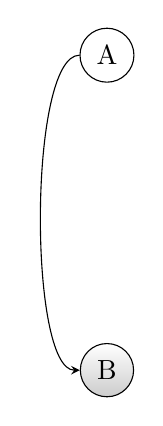
\begin{tikzpicture}[>=stealth]
	\node[circle,draw]  (A) at (0,4) {A};
	\node[circle,draw,top color=white,bottom color=black!20]  (B) at (0,0) {B};

	\draw[->] (A)  .. controls +(left:1) and +(left:1) ..  (B);
\end{tikzpicture}
\end{minipage}}
\hspace{1cm}
\subfigure[出站链路质量]{
\label{fig:subfig:b}
\begin{minipage}[b]{0.2\textwidth}
\centering
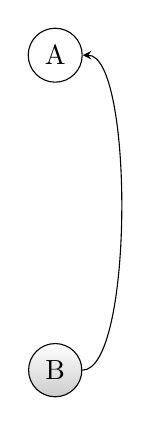
\begin{tikzpicture}[>=stealth]
	\node[circle,draw]  (A) at (0,4) {A};
	\node[circle,draw,top color=white,bottom color=black!20]  (B) at (0,0) {B};

	\draw[->] (B)  .. controls +(right:1) and +(right:1) ..  (A);
\end{tikzpicture}
\end{minipage}}
\hspace{1cm}
\subfigure[双向链路质量]{
\label{fig:subfig:c}
\begin{minipage}[b]{0.2\textwidth}
\centering
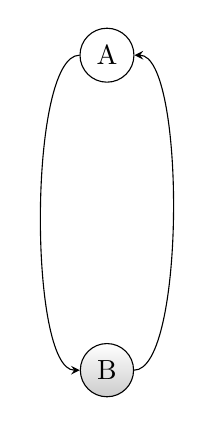
\begin{tikzpicture}[>=stealth]
	\node[circle,draw]  (A) at (0,4) {A};
	\node[circle,draw,top color=white,bottom color=black!20]  (B) at (0,0) {B};

	\draw[->] (A)  .. controls +(left:1) and +(left:1) ..  (B);
	\draw[->] (B)  .. controls +(right:1) and +(right:1) ..  (A);
\end{tikzpicture}
\end{minipage}}
\caption{三种链路质量}\label{link-quality}
\end{figure}


  \subsection{出站链路质量}
    如图\ref{fig:subfig:b}所示,节点对$(A,B)$,以B作为参考点,B向A发送帧数为$total_{out}$,
    其中A成功接收到帧数为$success_{out}$,从而有:
	\begin{equation}
		\text{\kai 出站链路质量} = \frac{success_{out}}{total_{out}}
	\end{equation}

    由于LEEP帧是通过广播方式发送的,节点B无法得知节点A是否收到,从而
    无法计算$success_{out}$。但B到A的出站链路质量即A到B的入站链路质量,要解决
    该问题只有让A把它与B间的入站链路质量回馈给B,这其实就是LEEP帧的主要
    功能之一。

    TinyOS 2.x中用8位无符号整数表示出站或入站链路质量。为了减少精度损失和
    充分利用8位的空间,TinyOS 2.x在实际存储该值时对它扩大255倍。

  \subsection{双向链路质量}
    如图\ref{fig:subfig:c}所示,对于有向节点对$(A,B)$,双向链路质量定义如下:
	\begin{equation}
		\text{\kai 双向链路质量} = \text{\kai 入站链路质量} \times \text{\kai 出站链路质量}
	\end{equation}

    本地干扰或噪声可以引起$(A,B)$和$(B,A)$链路质量不同,定义双向链路质量
    就是为了将这种情况考虑在内。
  \subsection{EETX值}
    TinyOS 2.x中使用EETX(Extra Expected number of Transmission)值表示双向链路质量估计值。
    在LEEP协议中使用的有两种EETX值:{\kai 窗口EETX}和{\kai 累积EETX}。窗口EETX是接收到的LEEP帧数或发送
    的数据包数达到一个固定的窗口大小时,根据窗口中的收发成功率计算出的EETX。而累积EETX则
    是本次窗口EETX和上次累积EETX加权相加得到的。根据指数移动平均的原理让旧值的权重逐渐减少,
    以适应链路质量的变化,是比较符合实际的统计方法。

\section{LEEP协议对数据链路层的要求}
\noindent LEEP协议对数据链路层有以下三个要求:
\vspace{-8pt}
\begin{enumerate}
	\item 有单跳源地址
	\item 提供广播地址
	\item 提供LEEP帧长度
\end{enumerate}
\vspace{-8pt}

  其中,有单跳源地址的要求是为了让收到广播LEEP帧的节点确定更新邻居表中哪一项
  的出站链路质量。现有节点的数据链路层一般都可以满足这3个要求。

\section{LEEP帧结构}
  根据以上分析可以得知LEEP帧至少应具备一个顺序号和与邻居节点间的入站链路质量。
  TinyOS 2.x中实现的LEEP帧结构如图\ref{leep-frame-structure}所示:
\begin{figure}[ht]
\centering

\begin{tikzpicture}
	\pagella
	\draw (0,0) rectangle (12,1);
	\foreach \x in {3,5,7,9,10,12}
	{
	  \draw (\x,0) -- (\x,1);
	}
	\foreach \x/\txt in {1.5/LEEP Header,4/Payload,6/LI Entry 1,8/LI Entry 2,9.5/\dots,11/LI Entry n}
	{
	  \draw (\x,0.5) node {\txt};
	}
\end{tikzpicture}
\caption{LEEP帧结构}\label{leep-frame-structure}
\end{figure}

  其中LEEP头部结构如图\ref{leep-frame-head}所示:

\begin{figure}[ht]
\centering
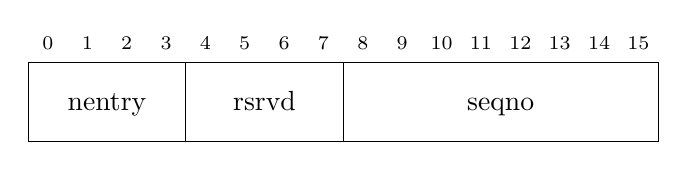
\begin{tikzpicture}
	\pagella
	\draw (0,0) rectangle (8,1);
	\foreach \x in {0,...,15}
	{
	  \draw (\x*0.5+0.25,1.25) node {\scriptsize \x};
	}
	\foreach \x in {2,4}
	{
	  \draw (\x,0) -- (\x,1);
	}
	\foreach \x/\txt in {1/nentry,3/rsrvd,6/seqno}
	{
	  \draw (\x,0.4) node[anchor=base] {\txt};
	}
\end{tikzpicture}
\caption{LEEP帧头部}\label{leep-frame-head}
\end{figure}

  各字段定义:
\vspace{-10pt}
\begin{itemize}
	\item nentry:尾部的LI项个数
	\item seqno:LEEP帧顺序号
	\item rsrvd:保留字段必须设为0
\end{itemize}
\vspace{-5pt}

    链路信息项格式如图\ref{link-info-frame}所示:

\begin{figure}[ht]
\centering
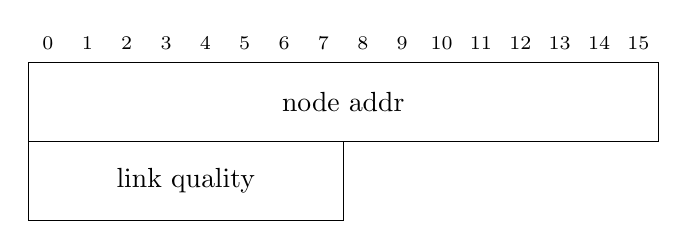
\begin{tikzpicture}
	\pagella
	\draw (0,0) rectangle (8,1);
	\foreach \x in {0,...,15}
	{
	  \draw (\x*0.5+0.25,1.25) node {\scriptsize \x};
	}
	\draw (4,0.5) node {node addr};
	\draw (0,0) -- (0,-1)--(4,-1)--(4,0);
	\draw (2,-0.5) node {link quality};
\end{tikzpicture}
\caption{链路信息项}\label{link-info-frame}
\end{figure}

    各字段定义如下:
\vspace{-10pt}
\begin{itemize}
	\item node addr:邻居节点的链路层地址
	\item link quality:从与node id对应的节点到本节点的入站链路质量
\end{itemize}

\section{实现}
  TinyOS中可选的链路估计器有两种:标准LE估计器和4位链路估计器。可以通过更改应用程序Makefile
中对应的路径选择使用哪一个链路估计器。
  \subsection{标准LE估计器}
  TinyOS 2.x中标准LE估计器的实现在\texttt{tos/lib/net/le}目录下:
\vspace{-10pt}
\begin{itemize}
  \item {\texttt{LinkEstimator.h}}:	头文件,包含了邻居表大小、邻居表项结构、LEEP帧头尾结构
  			以及LEEP协议中用到的常数的定义。
  \item {\texttt{LinkEstimator.nc}}:	接口定义。包含了其它组件可以从LinkEstimator中调用的方法。由如下代码所示,这些方法可以分三类,一类用于获取链路质量,一类用于操作邻居表,还有一类用于数据包估计。

%\begin{lstlisting}[captionpos=b,caption={LinkEstimator接口},label=linkestimator-h]
\begin{lstlisting}
interface LinkEstimator {
	command uint16_t getLinkQuality(uint16_t neighbor);
	command uint16_t getReverseQuality(uint16_t neighbor);
	command uint16_t getForwardQuality(uint16_t neighbor);

	command error_t insertNeighbor(am_addr_t neighbor);
	command error_t pinNeighbor(am_addr_t neighbor);
	command error_t unpinNeighbor(am_addr_t neighbor);

	command error_t txAck(am_addr_t neighbor);
	command error_t txNoAck(am_addr_t neighbor);
	command error_t clearDLQ(am_addr_t neighbor);

	event void evicted(am_addr_t neighbor);
}
\end{lstlisting}
  \item {\texttt{LinkEstimatorC.nc}}:	配置文件,用于说明链路估计器提供LinkEstimator接口。
  \item {\texttt{LinkEstimatorP.nc}}:	LEEP协议具体实现。
\end{itemize}
\vspace{-10pt}
  
    LEEP协议的目的是为了得到本节点到邻居节点间的双向链路质量。实现中使用两种策略
    相结合来计算估计值,两者间的关系如图\ref{ld-estimate}所示:
\begin{figure}[ht]
\centering
\begin{tikzpicture}[>=latex]
	\usetikzlibrary{shapes.multipart}
	\tikzstyle{rec}=[minimum width=1cm,minimum height=1cm,rectangle,draw]
	\draw (-1,6) node[text width=1.8cm,text centered] (A) {广播\\ EETX帧};
	\draw (-1,2) node[text width=2.8cm,text centered] (B) {转发引擎\\ACK接收情况};

	\node[rec] (WL) at (1.5,6) {窗口};
	\node[rec] (WD) at (1.5,2) {窗口};
	\node[rec] (L) at (3.5,6) {L估计};
	\node[rec] (D) at (3.5,2) {D估计};

	\node[rec] (EMA) at (5,4) {指数移动平均};
	\node[rec] (OEETX) at (7,1) {原EETX};
	\node[rec] (EETX) at (9,4) {累积EETX};

	\path (A) edge[->] (WL) ;
	\path (B) edge[->] (WD);
	\path (WL) edge[->] node[above]{\fontsize{9pt}{9pt}满} (L);
	\path (WD) edge[->] node[above]{\fontsize{9pt}{9pt}满} (D);
	\path (L) edge[->] (EMA);
	\path (D) edge[->] (EMA);
	\path (EMA) edge[->] (EETX);
	\path (EETX) edge[->] (OEETX);
	\path (OEETX) edge[->] (EMA);
	\node[rotate=56] at (8.3,2.4) {\fontsize{9pt}{9pt}下一次计算};
\end{tikzpicture}


\caption{链路估计值计算}\label{ld-estimate}
\end{figure}

    \subsubsection{根据LEEP帧的估计(L估计)}
      LEEP帧的估计通过LEEP帧的信息来估计EETX值。

      LEEP帧的发送:使用Send.send()方法,调用addLinkEstHeaderAndFooter()函数加LEEP
      	头尾。尾部存放的是本节点到邻居节点的链路质量表,如果LEEP帧中一次放不下
	这个表,则在下次发LEEP帧时从首个上次放不下的表项放起,以保证每个表项
	有平等的发送机会。每发一个包都将帧中的顺序号字段加1。
	发送的时机由LinkEstimator的使用者决定。

      LEEP帧的接收:每当收到一个LEEP帧,会触发SubReceive.receive()事件。
	处理程序根据LEEP头尾信息更新邻居表。这些操作集中在函数
      	processReceiveMessage()中进行,该函数找到这个LEEP帧发送者对应的邻居表项,调用
	updateNeighborEntryIdx()函数更新收到包数计数值和丢包数计数值。其中的丢包数就
	是本次与上次LEEP帧中顺序号字段的差值。

	当收到的包数达到一个固定窗口的大小时,
	调用updateNeighborTableEst()函数计算该窗口中的入站链路质量~$inquality_{win}$:
	\begin{equation}
      		inquality_{win} = 255 \times \frac{\text{\kai 接收到LEEP帧数}}{\text{\kai 总帧数}}
	\end{equation}
        根据动态移动平均原理更新入站链路质量:
	\begin{equation}
		inquality = \frac{\alpha \times inquality_{orig} + (10 - \alpha) \times inquality_{win}} {10}
	\end{equation}
	  TinyOS 2.x中设衰减系数$\alpha$值为9,因此每次更新时,旧值占$\frac{9}{10}$的权重,而新
	  值占$\frac{1}{10}$的权重。

	入站链路质量发生了变化,因此需要相应地计算双向链路质量。首先计算窗口EETX值~$EETX_{win}$:
	\begin{equation}
		EETX_{win} = (\frac{255^2}{inquality \times outquality} - 1) \times 10
	\end{equation}
	为了提高存储精度,EETX值都是扩大10倍存储。

	接着更新累积EETX值:
	\begin{equation}
		EETX = \frac{\alpha \times EETX_{orig} + (10-\alpha) \times EETX_{win}}{10}
	\end{equation}

    \subsubsection{根据数据包的估计(D估计)}
      根据数据包的估计通过发送数据包的成功率来估计EETX值。

      LinkEstimator并不能得知上层的数据包是否发送成功。因此它提供两个命令txAck()和txNoAck()
      让上层组件调用。txAck()用于告知链路估计器数据包发送成功,它将对应通信邻居的成功传输
      数据包计数值和总传输包计数值加1。当总传输包数达到一个固定窗口的大小时,调用updateDEETX()
      函数计算窗口EETX值~$DEETX_{win}$:
	\begin{equation}
      		DEETX_{win} = (\frac{\text{\kai 总包数}}{\text{\kai 成功包数}} - 1) \times 10
	\end{equation}
      接着更新累积EETX值:
	\begin{equation}
      		EETX = \frac{\alpha \times EETX_{orig} + (10-\alpha) \times DEETX_{win}}{10}
	\end{equation}

\subsection{四位链路估计(4BITLE)}
四位链路估计\ucite{fonseca2007fbw}与标准LE估计器的实现在结构上大体上是相同的。有所改进的是它提炼了物理层、链路层和网络层回馈的信息用于更精确的链路估计。其中1位来自物理层,1位来自链路层,2位来自网络层。4BITLE的实现在\texttt{tos/lib/net/4bitle}目录下。

\subsubsection{物理层}
在物理层,我们可以从一个包的传输中测量信道的质量。通常情况下,接收到错误位比较少的包很可能比错误多的包链路质量好。物理层的测量是快速并且廉价的,可以避免估计器在网络边缘或劣质的连接上浪费精力。我们可以把它提炼为一个white位,它表示在接收包时信道链路质量的优劣程度。

\subsubsection{链路层}
在链路层,我们可以测量包是否被传输并确认。基于广播探测的估计器面临着一个问题,它们将链路估计和数据通信分开实现,如果链路质量变坏导致包丢失,链路估计器要直到下一个路由信标被丢弃时才能反映这种变化。为了解决该问题,我们使用一个ack位,表示节点在一次传输中是否收到链路层的确认。

\subsubsection{网络层}
在网络层,我们可以了解到哪个连接是高层性能上最有价值的。如果没有网络层的信息,估计器可能选择一条路由环路,或者在最坏的情况下会与网络失去连接。无线传感器网络很可能会因链路层和网络层链路表的不一致而导致故障。我们可把这些提炼为2个位:
\vspace{-10pt}
  \begin{itemize}
	\item{pin位:} 用于告诉估计器不能剔除正在使用的连接。
	\item{compare位:} 用于告诉网络层这个连接看起来颇有希望。
  \end{itemize}

\subsection{链接质量指示(LQI)}
链接质量指示(Link Quality Indicator, LQI)是MultiHopLQI汇聚协议中用于链路估计的部分。它需要无线模块支持LQI,因此它只适用于CC2420之类具有链接质量指示器的节点。它完全使用物理层的信息作链路估计。

\chapter{路由引擎}\label{routing}

\section{简介}

路由引擎的责任是选择传输的下一跳。一个理想的路由引擎应当可以选择到根节点跳数尽量少而连接质量尽量好的传输路径,这样可以减少转发次数和丢包率,从而降低传感器网络的能量消耗,延长网络的生存期。但由于节点的的存储容量和处理能力一般都非常有限,难以存储大量的路由信息和使用复杂的路由算法,故而有线网络中常用的路由算法如TCP/IP中的OSPF和RIP协议\ucite{stevens1993tii}在这里是不适用的。传感器网络的路由设计注重简单有效,使用有限的资源达到最好的效果。TinyOS 2.x中CTP协议实现的路由引擎可以较好地实现这个目标。它用于建立到根节点的汇聚树,利用链路质量估计器提供的信息合理地选择下一跳节点,使采样节点到根节点的传输次数尽可能地少。

\section{基本概念}
\subsection{路径ETX}
路径ETX(Expected number of Transmissions)是父节点到根节点的ETX与本节点与父节点间的单跳ETX之和,如图\ref{etx-tree}所示。单跳ETX与链路估计器提供的EETX值关系为ETX=EETX+1。它的大小可以反映出到根节点的跳数。在一般情况下,路径ETX越小说明离根节点越近,路由引擎正是根据这一事实选择ETX最小的邻居作为父节点,以期获得到根节点的最少传输次数。
\begin{figure}[ht]
\centering
\begin{tikzpicture}[grow=right, sloped]
\tikzstyle{level 1}=[level distance=3.5cm, sibling distance=3.5cm]
\tikzstyle{level 2}=[level distance=3.5cm, sibling distance=2cm]

\tikzstyle{bag} = [text width=2em, text centered,draw,circle,inner sep=0pt]
\tikzstyle{end} = [circle, minimum width=3pt,fill, inner sep=0pt]
\usetikzlibrary{trees}
\node[bag] {$0$}
    child {
        node[bag] {$4$}        
            child {
                node[end, label=right:
                    {$8$}] {}
                edge from parent
                node[above] {$$}
                node[below]  {$4$}
            }
            child {
                node[end, label=right:
                    {$9$}] {}
                edge from parent
                node[above] {$$}
                node[below]  {$5$}
            }
            edge from parent 
            node[above] {$$}
            node[below]  {$4$}
    }
    child {
        node[bag] {$3$}        
        child {
                node[end, label=right:
                    {$6$}] {}
                edge from parent
                node[above] {$$}
                node[below]  {$3$}
            }
            child {
                node[end, label=right:
                    {$9$}] {}
                edge from parent
                node[above] {$$}
                node[below]  {$6$}
            }
        edge from parent         
            node[above] {$$}
            node[below]  {$3$}
    };
\end{tikzpicture}

\caption{路径ETX值计算}\label{etx-tree}
\end{figure}
\subsection{路由表}
路由表是路由引擎的核心数据结构。CTP协议中使用的路由表结构如图\ref{route-table}所示的形式,它存储了邻居节点信息,主要是邻居的路径ETX值。路由表的大小取决于链路估计器邻居表的大小,因为不在邻居表的节点无法作为邻居节点进入路由表。

\begin{figure}
\centering
\begin{tabular}{|c|c|c|c|}
\hline
\raisebox{-15pt}{邻居节点地址} &\multicolumn{3}{c|}{\raisebox{-8pt}{路由信息}} \\ \cline{2-4}
 &父节点地址 & ETX &  拥塞 \\
\hline
0&&& \\
\hline
1&&& \\
\hline
2&\ldots &\ldots &\ldots  \\
\end{tabular}
\caption{路由表结构}\label{route-table}
\end{figure}


\subsection{CTP路由帧(信标帧)}
路由引擎用广播的形式发送路由帧以便在节点间交换路由信息。

CTP路由帧格式如图\ref{ctp-route-frame}所示:

\begin{figure}[ht]
\centering
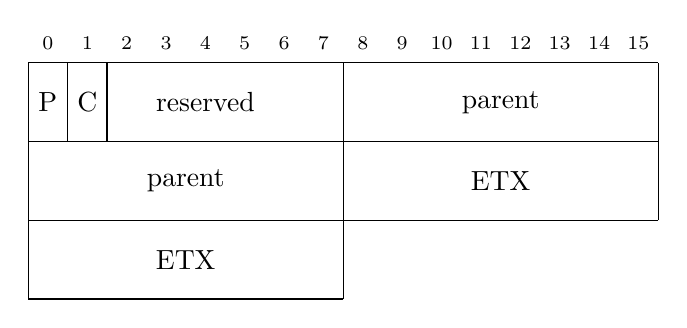
\begin{tikzpicture}
	\pagella
	\draw (0,0) -- (4,0);
	\draw (0,1) -- (8,1);
	\draw (0,2) -- (8,2);
	\draw (0,3) -- (8,3);

	\draw (0,0) -- (0,3);
	\draw (0.5,2) -- (0.5,3);
	\draw (1,2) -- (1,3);
	\draw (4,0) -- (4,3);
	\draw (8,1) -- (8,3);
	\foreach \x in {0,...,15}
	{
	  \draw (\x*0.5+0.25,3.25) node {\scriptsize \x};
	}
	\draw (0.25,2.5) node {P};
	\draw (0.75,2.5) node {C};
	\draw (2.25,2.5) node {reserved};
	\draw (6,2.5) node {parent};
	\draw (2,1.5) node {parent};
	\draw (6,1.5) node {ETX};
	\draw (2,0.5) node {ETX};
\end{tikzpicture}
\caption{CTP路由帧格式}\label{ctp-route-frame}
\end{figure}

各字段意义如下:
\vspace{-10pt}
\begin{itemize}
	\item P:取路由位。如果节点收到一个P位置位的包,它应当尽快传输一个路由帧。
	\item C:拥塞标识。如果节点丢弃了一个CTP数据帧,则必须将下一个传输路由帧的C位置位。
	\item parent:节点的当前父节点
	\item ETX:节点的当前ETX值
\end{itemize}
\vspace{-10pt}
当节点接收到一个路由帧时,它必须更新路由表相应地址的ETX值。如果节点的ETX值变动很大,那么CTP必须传输一个广播帧以通知其它节点更新它们的路由。与CTP数据帧相比,路由帧用父节点地址代替了源节点地址。父节点可能发现子节点的ETX值远低于自己的ETX值的情况,这时它需要准备尽快传输一个路由帧。

\subsection{当前路由信息}
记录当前使用的父节点的信息。如它的AM层地址,路径ETX等。

\section{实现}
TinyOS中路由引擎的实现在\texttt{tos/lib/net/ctp}目录的下列文件中:

\vspace{-10pt}
\begin{itemize}
	\item \texttt{CtpRoutingEngineP.nc}: 路由引擎的具体实现
	\item \texttt{TreeLouting.h}: 路由引擎中使用的一些结构和常数的定义
	\item \texttt{Ctp.h}: 路由帧结构的定义
\end{itemize}
\vspace{-10pt}

\subsection{使用的接口和提供的组件}
从下列源码中可以看到,CtpRoutingEngineP是一个通用组件,可以通过参数设定路由表大小、信标帧发送的最小和最大间隔。它使用了链路估计器、两个定时器和一些包收发处理接口;提供的接口主要是Routing路由接口,它包含了一个最重要的命令nexthop()用于为上层组件提供下一跳的信息。

%\begin{lstlisting}[captionpos=b,caption={\song CtpRoutingEngineP组件使用和提供的接口},label=ctp-routing-engine]
\begin{lstlisting}
generic module CtpRoutingEngineP(uint8_t routingTableSize, 
				uint32_t minInterval, uint32_t maxInterval) {
	provides {
		interface UnicastNameFreeRouting as Routing;
		interface RootControl;
		interface CtpInfo;
		interface StdControl;
		interface CtpRoutingPacket;
		interface Init;
	} 
	uses {
		interface AMSend as BeaconSend;
		interface Receive as BeaconReceive;
		interface LinkEstimator;
		interface AMPacket;
		interface SplitControl as RadioControl;
		interface Timer<TMilli> as BeaconTimer;
		interface Timer<TMilli> as RouteTimer;
		interface Random;
		interface CollectionDebug;
		interface CtpCongestion;

		interface CompareBit;
	}
}
\end{lstlisting}

\subsection{信标帧定时器与路由定时器}
	\subsubsection{信标帧定时器}
	信标帧定时器(BeaconTimer)用于周期性的发送信标帧。发送间隔是指数级增长的。初始的间隔是一个常数minInterval(其值为128),在每更新一次路由信息后,将间隔加倍。因此随着网络的逐渐稳定,将很少看到节点广播信标帧。定时器间隔在使用指数级增长的基础上还加上随机数以错开发送信标帧的时机,避免节点同时发送信标帧导致信道冲突。此外,定时器可以重置为初始值,这主要用于处理一些特殊情况,比如节点收到一个P位置位的包要求尽快发信标帧,或者提供给上层使用者重置间隔的功能。
	\subsubsection{路由定时器}
	路由定时器(RouteTimer)用于周期性的启动更新路由任务。更新间隔固定为一个常数BEACON\_INTERVAL,其值为8192。该定时器触发后将启动更新路由选择任务。

\subsection{发送信标帧与更新路由选择任务}
	\subsubsection{发送信标帧任务}
	由信标帧定时器触发。以广播的方式告知其它节点本节点的ETX值、当前父节点和拥塞信息。
	\subsubsection{更新路由选择任务}
	更新路由选择任务一般由路由定时器触发,但也可以在其它条件下触发,如信标帧定时器到期、重新计算路由、剔除了某个邻居等需要更新路由选择的情况下触发。更新路由选择任务通过遍历路由表找出路径ETX值最小的节点作为父节点,并且该节点不能是拥塞的或是本节点的父节点。

\subsection{信标帧接收事件}
BeaconReceive.receive()事件,在收到其它节点的信标帧时触发。它将根据信标帧的发送者和ETX值更新相应的路由表项。如果收到的是根节点的信标帧,则调用链路估计器将它固定在连接表中。如果信标帧的P位置位,则重设信标帧定时器,以便尽快广播本节点的信标帧让请求者收到。

\subsection{工作流程分析}

路由引擎工作流程如图\ref{route-engine}所示。节点启动时将初始化路由引擎。路由引擎通过将Init接口接到MainC的SoftwareInit接口以实现节点启动时自动初始化路由引擎。初始化的工作有:初始化当前路由信息、初始化路由表为空,初始化路由帧消息缓冲区以及一些状态变量等。

应用程序通过StdControl接口的start()方法正式启动路由引擎,这将启动两个定时器RouteTimer和BeaconTimer。其中RouteTimer的时间间隔设为BEACON\_INTERVAL(8192),BeaconTimer的下一次发送时间初始值设为minInterval(128)。

\begin{figure}[ht]
\centering
\begin{tikzpicture}[>=latex,scale=1.4]
	\draw[->] (0,5.7) -- (0.7,5.7);
	\draw[->] (0,5.7) -- (0,6.3);
	\draw (0,5.8) parabola (0.6,6.2);

	\draw[->] (0,3.7) -- (0.7,3.7);
	\draw[->] (0,3.7) -- (0,4.3);
	\draw (0,3.95) -- (0.6,3.95);

	\draw (1.5,6) circle (0.3);
	\draw (1.5,6) -- (1.8,6);
	\draw (1.5,6) -- (1.5,6.3);

	\draw (1.5,4) circle (0.3);
	\draw (1.5,4) -- (1.8,4);
	\draw (1.5,4) -- (1.5,4.3);

	\draw[->,gray,line width=2pt] (3-0.3,6) -- (3+0.3,6);
	\draw[->,gray,line width=2pt] (3-0.3,4) -- (3+0.3,4);

	\draw (3.5,6.3) rectangle (4.5,5.7);
	\draw (3.8,6.3) -- (3.8,5.7);

	\draw (3.5,3) -- (3.5,4.5) -- (5,4.5) -- (5,3);
	\draw (3.5,3.3) -- (5,3.3);
	\draw (3.5,3.6) -- (5,3.6);
	\draw (3.5,3.9) -- (5,3.9);
	\draw (3.5,4.2) -- (5,4.2);

	\draw (3.9,4.5) -- (3.9,3);
	\draw (4.5,4.5) -- (4.5,3);
	\node at (4.2,4.35) {\tiny ETX};
	\node at (4.2,4.05) {\tiny 9};
	\node at (4.2,3.75) {\tiny 6};
	\node at (4.2,3.45) {\tiny 4};
	\node at (3.7,4.05) {\tiny 2};
	\node at (3.7,3.75) {\tiny 5};
	\node at (3.7,3.45) {\tiny 3};
	\node at (3.7, 3.15) {\tiny\ldots};
	\node at (4.2, 3.15) {\tiny\ldots};
	\node at (4.75, 3.15) {\tiny\ldots};

	\node[draw, circle] (parent) at (5.9,4) {3};
	\node[inner sep=1,circle,fill] (d) at (4.75,3.45) {};
	\draw[->] (d) .. controls +(right:1) and +(left:1) .. (parent);

	\draw[dashed] (7,7) -- (7,2);

	\draw (8,6.3) rectangle (9,5.7);
	\draw (8.3,6.3) -- (8.3,5.7);

	\draw (8,3) -- (8,4.5) -- (9.5,4.5) -- (9.5,3);
	\draw (8,3.3) -- (9.5,3.3);
	\draw (8,3.6) -- (9.5,3.6);
	\draw (8,3.9) -- (9.5,3.9);
	\draw (8,4.2) -- (9.5,4.2);

	\draw (8.4,4.5) -- (8.4,3);
	\draw (9,4.5) -- (9,3);
	\node at (8.7,4.35) {\tiny ETX};
	\node at (8.2,4.05) {\tiny 4};
	\node at (8.2,3.75) {\tiny 1};
	\node at (8.2,3.45) {\tiny 3};
	\node at (8.2, 3.15) {\tiny\ldots};
	\node at (8.7, 3.15) {\tiny\ldots};
	\node at (9.25, 3.15) {\tiny\ldots};

	\node[inner sep=1,fill,circle] (head) at (8.15,6) {};
	\node[inner sep=0] (end) at (8,3.75) {};
	\draw[->] (head) .. controls +(left:1) and +(left:1) .. (end);

	\draw (2.2,6.15) node[text width=1cm,text centered] {\scriptsize 信标帧};
	\draw (2.2,5.85) node[text width=1cm,text centered] {\scriptsize 定时器};
	\draw (2.2,4.15) node[text width=1cm,text centered] {\scriptsize 路由};
	\draw (2.2,3.85) node[text width=1cm,text centered] {\scriptsize 定时器};
	\draw (4.35,4.7) node[text width=1cm,text centered] {\scriptsize 路由表};
	\draw (8.85,4.7) node[text width=1cm,text centered] {\scriptsize 路由表};
	\draw (4,6.5) node[text width=1cm,text centered] {\scriptsize 信标帧};
	\draw (8.5,6.5) node[text width=1cm,text centered] {\scriptsize 信标帧};
	\draw (6,3.15) node[text width=2cm,text centered] {\scriptsize 选择ETX最小};
	\draw (6,2.85) node[text width=2cm,text centered] {\scriptsize 的作为父节点};
	\draw (7.5,3.15) node[text width=1cm,text centered] {\scriptsize 更新路};
	\draw (7.5,2.85) node[text width=1cm,text centered] {\scriptsize 由表项};
	\draw (2,2.4) node {节点1};
	\draw (9,2.4) node {节点2};

	\draw[->,gray,line width=1.5pt] (5,6) -- (7.5,6);
\end{tikzpicture}

\caption{路由引擎工作流程}\label{route-engine}
\end{figure}

由于BeaconTimer的触发时间值设置的比RouteTimer的触发间隔小的多,因此BeaconTimer将率先触发,并投递updateRouteTask()以更新路由选择,接着投递sendBeaconTask()任务发送信标帧。此后,RouteTimer以恒定的时间间隔触发并投递updateRouteTask(),而BeaconTimer触发后会将下次触发的时间间隔加倍。

除了定时器在不断的触发以投递任务外,路由引擎还需要处理其它节点的信标帧。当接收到一个广播的信标帧时,会触发BeaconReceive.receive()事件并根据信标帧中的发送者和它的ETX值更新相应的路由表项。

另外,如果链路估计器剔除了一个侯选邻居,则路由引擎也要相应地从路由表把该邻居移除,并更新路由选择,从而保证了路由表和连接表的一致性。


\chapter{转发引擎}\label{forward}

\section{简介}
转发引擎主要负责以下5种工作:
\vspace{-8pt}
\begin{enumerate}
	\item 向下一跳传递包,在需要时重传,同时根据是否收到ACK向链路估计器传递相应信息。
	\item 决定何时向下一跳传递包
	\item 检测路由中的不一致性,并通知路由引擎
	\item 维护需要传输的包队列,它混杂了本地产生的包和需要转发的包。
	\item 检测由于丢失ACK引起的单跳重复传输
\end{enumerate}

\section{基本概念}
\subsection{路由循环}
路由循环是指某个节点将数据包转发给下一跳,而下一跳节点是它的子孙节点或者它本身,从而造成了数据包
在该环路中不断循环传递,如图\ref{route-loop}所示,由于节点E在某个时刻错误地选择了H节点作为父节点,从而造成了路由循环。

\begin{figure}[ht]
\centering
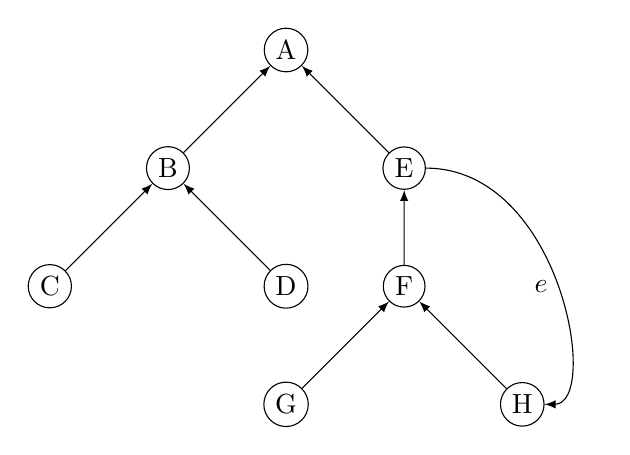
\begin{tikzpicture}[>=latex,level/.style={sibling distance=3cm}]
	\node[circle,draw,inner sep=2] {A}
		child[<-] {node[circle,draw,inner sep=2] {B}
			child {node[circle,draw,inner sep=2] {C}}
			child {node[circle,draw,inner sep=2] {D}}
		}
		child[<-] {node[circle,draw,inner sep=2] (E) {E}
			child {node[circle,draw,inner sep=2] {F}
				child {node[circle,draw,inner sep=2] {G}}
				child {node[circle,draw,inner sep=2] (H) {H}}
			}
		};
	\draw[->] (E) .. controls +(right:2) and +(right:1) .. node[left] {$e$}(H);
\end{tikzpicture}


\caption{路由循环}\label{route-loop}
\end{figure}

\subsection{包重复}
包重复是指节点多次收到具有相同内容的包。这主要是由于包重传引起的。比如发送者发送了一个数据包,
接收者成功地收到了该数据包并回复ACK,但ACK在中途丢失,因此发送者会将该包再一次发送,从而在
接收者处造成了包重复现象。

\subsection{CTP数据帧}
CTP数据帧是转发引擎在发送本地数据包时所使用的格式。它在数据包头增加一些字段用于抑制包重复和路由循环。

CTP数据帧格式如图\ref{ctp-data-frame}所示:
\begin{figure}[ht]
\centering
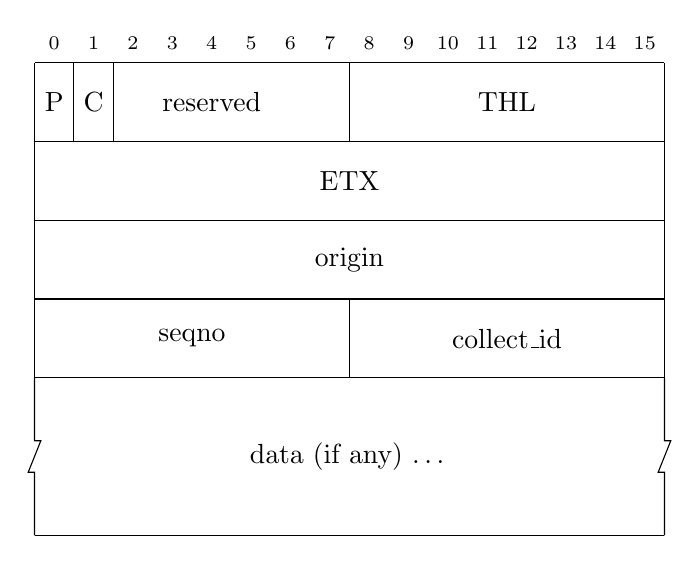
\begin{tikzpicture}
\pagella
	\draw (0,-1) -- (8,-1);
	\draw (0,1) -- (8,1);
	\draw (0,2) -- (8,2);
	\draw (0,3) -- (8,3);
	\draw (0,4) -- (8,4);
	\draw (0,5) -- (8,5);

	\draw (0,1) -- (0,5);
	\draw (8,1) -- (8,5);

	%\draw (0,0) -- (0,0.4) -- (-0.08,0.4) -- (0.08,0.6) -- (0,0.6) -- (0,1);
	\draw (0,-1) -- (0,-0.2) -- (-0.08,-0.2) -- (0.08,0.2) -- (0,0.2) -- (0,1);
	%\draw (8,0) -- (8,0.4) -- (8-0.08,0.4) -- (8+0.08,0.6) -- (8,0.6) -- (8,1);
	\draw (8,-1) -- (8,-0.2) -- (8-0.08,-0.2) -- (8+0.08,0.2) -- (8,0.2) -- (8,1);

	\draw (0.5,4) -- (0.5,5);
	\draw (1,4) -- (1,5);
	\draw (4,4) -- (4,5);
	\draw (4,1) -- (4,2);

	\foreach \x in {0,...,15}
	{
	  \draw (\x*0.5+0.25,5.25) node {\scriptsize \x};
	}
	\draw (0.25,4.5) node {P};
	\draw (0.75,4.5) node {C};
	\draw (2.25,4.5) node {reserved};
	\draw (6,4.5) node {THL};
	\draw (4,3.5) node {ETX};
	\draw (4,2.5) node {origin};
	\draw (2,1.5) node {seqno};
	\draw (6,1.5) node {collect\_id};
	\draw (4,0) node {data (if any) \ldots};
\end{tikzpicture}
\caption{CTP数据帧格式}\label{ctp-data-frame}
\end{figure}

各字段定义如下:
\vspace{-10pt}
\begin{itemize}
	\item P:取路由位。P位允许节点从其它节点请求路由信息。
		如果节点收到一个P位置位的包,它应当传输一个路由帧。
	\item C:拥塞标志位。如果节点丢弃了一个CTP数据帧,
		它必须在下一个传输的数据帧中置C位。
	\item THL:已存活时间(Time Have Lived),它主要用于解决路由循环问题。
		当节点产生一个CTP数据帧时,
		它必须设THL为0。当节点接收到一个CTP数据帧时,
		它必须增加THL值。如果节点接收到的数据包THL为255,则将它回绕为0。
		该字段主要用于解决数据包在环路中停留太久的问题,
		但在当前版本的CTP协议中暂时还没有实现这一功能。
	\item ETX:单跳发送者的ETX值。当节点发送一个CTP数据帧时,
		它必须将到单跳目的地的路由ETX值填入ETX字段。
		如果节点接收到的路由梯度比自己的小,则它必须准备发送一个路由帧。
	\item origin:包的源地址。转发的节点不可修改这个字段。
	\item seqno:源顺序号。源节点设置了这个字段,转发节点不可修改它。
	\item collect\_id:高层协议标识。源节点设置了这个字段,转发节点不可修改它。
	\item data:数据负载。0个或多个字节。转发节点不可修改这个字段。
\end{itemize}
\vspace{-10pt}

origin,~seqno,~collect\_id合起来标识了一个唯一个源数据包,
而origin,~seqno,~collect\_id,~THL合起来标识了网络中唯一一个数据包实例。
两者的区别在路由循环中的重复抑制是很重要的。如果节点抑制源数据包,
则它可能丢弃路由循环中的包;如果它抑制包实例,则它允许转发处于短暂
的路由循环中的包,除非THL凑巧回绕到与上次转发时相同的状况。

\subsection{队列项}
队列项(Queue Entry)中存放了对应消息的指针、对应的发送者和可重传次数。本地包与转发包的队列项分配方法有所不同:转发包的队列项是通过缓冲池分配的,而本地包的队列项是编译期间静态分配的。

\subsection{消息发送队列}
消息发送队列结构是转发引擎的核心结构。它存放了队列项的指针,
队头元素指向的队列项中的消息将被优先发送。

\subsection{缓冲池}
缓冲池是操作系统中用于统一管理缓冲区分配的一个设施\ucite{bach1986duo}。
应用程序可以使用缓冲池提供的接口方便地获取和释放缓冲区。
对于不能动态分配存储空间的TinyOS来说,这一点非常有价值,因为它可以重复
利用一段静态存储空间。

转发引擎中使用了两个缓冲池:队列项缓冲池(QEntryPool)和消息缓冲池
(MessagePool)。队列项缓冲池用于为队列项分配空间,如图\ref{qe-buffer-pool}所示,
当转发引擎收到一个需要转发的消息时,它会从队列项缓冲区中取出一个空闲的队列项,
作相应的初始之后把队列项的指针放入消息队列队尾。在成功地发送了一个
消息并收到ACK或消息重发次数过多被丢弃时,转发引擎会从队列项缓冲池中
释放这个消息对应的队列项,使它变为空闲,因此队列缓冲池就可以把这块
空间分配给后续的消息。

\begin{figure}[ht]
\centering
\begin{tikzpicture}[>=latex]
	\fill[gray!40] (2,4) rectangle (3,3.5);
	\fill[gray!40] (2,2.5) rectangle (3,2);
	\draw (2,4) rectangle (3,2);
	\draw (2,2.5)--(3,2.5);
	\draw (2,3)--(3,3);
	\draw (2,3.5)--(3,3.5);
	\node at (2.5,3.75) {0};
	\node at (2.5,3.25) {1};
	\node at (2.5,2.75) {2};
	\node at (2.5,2.25) {3};

	\fill[gray!40] (7,3.5) rectangle (8,3);
	\fill[gray!40] (7,2) rectangle (8,1.5);
	\fill[gray!20] (7,2.5) rectangle (8,2);
	\draw (7,3.5) rectangle (8,1.5);
	\draw (7,3)--(8,3);
	\draw (7,2.5)--(8,2.5);
	\draw (7,2)--(8,2);
	\node at (7.5,3.25) {0};
	\node at (7.5,2.75) {1};
	\node at (7.5,2.25) {2};
	\node at (7.5,1.75) {3};

	\fill[gray!40] (5,8) rectangle (6,7.5);
	\fill[gray!40] (5,6.5) rectangle (6,6);
	\fill[gray!40] (5,7) rectangle (6,6.5);
	\draw (5,8) rectangle (6,6);
	\draw (5,7.5)--(6,7.5);
	\draw (5,7)--(6,7);
	\draw (5,6.5)--(6,6.5);
	\node at (5.5,7.75) {0};
	\node at (5.5,7.25) {1};
	\node at (5.5,6.75) {2};
	\node at (5.5,6.25) {3};
	
	%\draw[rotate=-10] (2,3.4) ellipse (1.2 and 1.5);
	%\draw[rotate=-10] (7,3.7) ellipse (1.2 and 1.5);
	%\draw[rotate=-10] (4.2,7.8) ellipse (1.2 and 1.5);

	\node (AI) at (2,2.75) {};
	\node (AO) at (3,2.75) {};
	\node (BI) at (7,2.25) {};
	\node (BO) at (8,2.25) {};
	\node (CI) at (6,6.6) {};
	\node (CO) at (5,6.75) {};

	\draw[->] (AO) .. controls +(right:2) and +(left:1) .. node[below] {获取qe} (BI);
	\draw[->] (BO) .. controls +(right:2) and +(right:2) .. node[right] {使用qe} (CI);
	\draw[->] (CO) .. controls +(left:2) and +(left:2) .. node[left] {释放qe} (AI);

	\draw (7,7.3) -- node[above] {\footnotesize 将qe指针放入发送队列} (9,7.3);
	\draw (7,6.7) -- (9,6.7);
	\draw (7.5,7.3) -- (7.5,6.7);
	\draw (7.9,7.3) -- (7.9,6.7);
	\draw (8.3,7.3) -- (8.3,6.7);
	\draw (8.7,7.3) -- (8.7,6.7);
	\node at (7.7,7) {2};
	\node at (8.1,7) {0};
	\node at (8.5,7) {3};
	\draw[->] (6,6.8) .. controls +(right:0.8) and +(left:0.5).. (7.3,7);
\end{tikzpicture}

\caption{从缓冲池分配和释放队列项}\label{qe-buffer-pool}
\end{figure}

消息缓冲池的工作原理与队列项缓冲池类似,只不过它存的是消息结构。
消息缓冲池有一个缓冲区交换的行为,在“缓冲区交换”一节中详细论述。

在TinyOS 2.x中,消息缓冲池的初始大小设定为一个常数FORWARD\_COUNT(值为12)。
队列项缓冲池的初始大小为CLIENT\_COUNT + FORWARD\_COUNT,
其中CLIENT\_COUNT是CollectionSenderC使用者的个数,加上它是考虑到了本地
产生的包也会进入发送队列,而本地包的最大个数正是CollectionSenderC使用者
的个数,这样就保证了发送队列不会因为本地发送者太多而不断产生溢出。
如果不考虑这个因素,则在本地发送者很多的情况下节点可能产生拥塞的假象。

\subsection{缓冲区交换}\label{bufswap}
缓冲区交换是转发过程中一个比较微妙的环节。如图\ref{buffer-swap}所示,
从缓冲池中获得的消息结构并不是直接用于存储当前接收到的消息,而是用于
存储下一次收到的消息。由于当前接收到的消息必定已经有了它自己的存储空间,
因此只要让相应的队列项指向它就可以找到这个消息的实体。但是下一个接收到的消息就不应该
存储在这一块空间,而缓冲区交换正是用于为下一次收到的消息分配另外一块
空闲的存储空间。传统的做法通常是设置一个消息结构用于接收消息,
每当收到一个消息后将它整个复制到空闲存储空间中。相比之下,缓冲区交换
可以省去一次复制的开销。

\begin{figure}[ht]
\centering
\begin{tikzpicture}[>=latex]
	\usetikzlibrary{shapes}
	\node[ellipse,draw] (BP) at (4,1.5) {缓冲池};
	\node[ellipse,draw] (MP) at (8,3.5) {队列项};
	\node[rectangle,draw] (BF) at (4,5.5) {缓冲区};
	\node[rectangle,draw] (RC) at (4,7) {接收器};

	\draw[->] (BP) .. controls +(left:2)  and +(left:2) .. node[left] {获取msg} (BF);
	\draw[->] (BF) .. controls +(right:2) and +(up:1.5) .. node[above,rotate=-20] {使用msg} (MP);
	\draw[->] (MP) .. controls +(down:1) and +(right:2) .. node[below,rotate=30] {释放msg} (BP);
	\draw[->] (RC) -- node[right] {填充msg} (BF);
\end{tikzpicture}

\caption{缓冲区交换}\label{buffer-swap}
\end{figure}

\section{实现}
组件\texttt{tos/lib/net/ctp/CtpForwardingEngineP.nc}实现了转发引擎。

\subsection{使用的接口和提供的组件}
从下列源码中可以看到,CtpForwardingEngine使用了路由引擎提供的接口UnicastNameFreeRouting用于得到下一跳信息,使用了系统提供的Queue、Pool、SendCache接口分别实现消息发送队列、队列项缓冲池、消息缓冲池和发送消息缓存,同时也使用了LinkEstimator用于向链路估计器反馈数据包发送成功与否的信息。

%\begin{lstlisting}[captionpos=b,caption={\song CtpForwardingEngineP组件使用和提供的接口},label=ctp-forward-engine]
\begin{lstlisting}
generic module CtpForwardingEngineP() {
	provides {
		interface Init;
		interface StdControl;
		interface Send[uint8_t client];
		interface Receive[collection_id_t id];
		interface Receive as Snoop[collection_id_t id];
		interface Intercept[collection_id_t id];
		interface Packet;
		interface CollectionPacket;
		interface CtpPacket;
		interface CtpCongestion;
	}
	uses {
		interface AMSend as SubSend;
		interface Receive as SubReceive;
		interface Receive as SubSnoop;
		interface Packet as SubPacket;
		interface UnicastNameFreeRouting;
		interface SplitControl as RadioControl;
		interface Queue<fe_queue_entry_t*> as SendQueue;
		interface Pool<fe_queue_entry_t> as QEntryPool;
		interface Pool<message_t> as MessagePool;
		interface Timer<TMilli> as RetxmitTimer;
		interface LinkEstimator;
		interface Timer<TMilli> as CongestionTimer;
		interface Cache<message_t*> as SentCache;
		interface CtpInfo;
		interface PacketAcknowledgements;
		interface Random;
		interface RootControl;
		interface CollectionId[uint8_t client];
		interface AMPacket;
		interface CollectionDebug;
		interface Leds;
	}
}
\end{lstlisting}

CtpForwardingEngine提供的接口分别为网络中的四种扮演不同角色的节点服务。为发送者提供Send接口,为侦听者提供Snoop接口,为网络处理者提供Intercept接口,为接收者提供Receive接口。

\subsection{关键函数}
转发引擎的四个关键函数为包接收SubReceive.receive(),包转发forward(),
包传输SendTask()和包传完之后的善后工作SubSend.sendDone()。

\subsubsection{receive()函数}
receive()函数决定节点是否转发一个包。它有一个缓冲区缓存了最近收到的包,
通过检查这个缓冲区可以确定它是否是重复的。如果不是,则调用forward()函数
进行转发。

\subsubsection{forward()函数}
forward()函数格式化需要转发的包。它检查收到的包是否有路由循环,使用的方法是判断包头中的ETX值是否比本节点的路径ETX小。接着检查发送队列中是否有足够的空间,如果没有,则丢弃该包并置C位。如果传输队列为空,则投递SendTask任务准备发送。

\subsubsection{SendTask任务}
SendTask任务检查位于发送队列队头的包,请求路由引擎的路由信息,为到下一跳的传输作好准备,
并将消息提交到AM层。

\subsubsection{sendDone事件}
当发送结束时,sendDone事件处理程序会检查发送的结果。如果包被确认,则将包从传输队列中取出。
如果包是本地产生的,则将sendDone信号向上传。如果包是转发的,则将该消息结构释放到
消息缓冲池。如果队列中还有剩余的包(比如没有被确认的),它启动一个随机定时器
以重新投递这个任务。该定时器实质上用于限制CTP的传输速率,不让它尽快地发包,
这是为了防止在通路上自我冲突。

\subsection{工作流程分析}
当转发引擎收到一个转发包时,它会检查该数据包是否在缓存或发送队列中,
这主要是为了抑制包重复。如果不是重复包,则调用forward()进行转发。forward()函数为该消息
在消息池中分配队列项和消息结构,然后把队列项指针放入发送队列。如果此时投递
发送消息任务的定时器没有运行,则立即投递发送消息任务,
以选取发送队列队头的数据包进行发送。发送成功之后将触发sendDone
事件做一些善后工作,比如检查刚发送的包是否收到链路层ACK,
如果收到,则从队列中删除这个包的队列项,并释放相关资源。如果
没有收到ACK,则启动重传定时器,再一次投递发送消息任务进行重传。
若重传次数超过CLIENT\_COUNT次,则丢弃该包。

\subsection{本地数据包的发送}
转发引擎也负责本地数据包的发送。应用程序通过使用CollectionSenderC
组件发送本地包。nesC编译器会根据CollectionSenderC组件使用者的
个数为每个使用者静态地分配一个队列项,并用一个指针数组指向各自的队列项。
如果某个使用者需要发送数据包,则先检查它对应的指针是否为空。若为空,
则说明该使用者发送的前一个数据尚未处理完毕,返回发送失败;若不为空,
则说明它指向的队列项可用,用数据包的内容填充队列项并把它放入发送队列等待发送。

\chapter{仿真与部署}\label{simulate}

\section{仿真}
\subsection{TOSSIM简介}
TOSSIM\ucite{levis2003taa}是一个TinyOS程序仿真工具。它是一个库,你可以写程序调用并运行以实现仿真。TOSSIM支持两种编程接口:Python和C++。Python可以交互式动态地仿真,如同一个强力的调试器。如果对仿真的时间性能要求较高,则可以用C++接口。

TOSSIM的工作原理是通过替换系统组件实现仿真,具体替换哪个组件视情况而定。比如定时器的仿真可以使用替换HilTimerMillic组件的方法实现,也可以通过替换atmega128平台硬件时钟的HPL(Hardware Presentation Layer)实现。前者是对任何平台通用的,但是缺乏逼真度。后者通过仿真芯片的行为实现,逼真度高,但是只对atmega128适用。TOSSIM是一个离散事件仿真器,它从事件队列(以发生时间排序)中取出事件并运行之。仿真事件可以是底层硬件中断或高层的系统事件(如包接收事件),也可以是任务。

\subsection{仿真CTP协议}
我们使用TinyOS 2.x中自带的示例\texttt{apps/tests/TestNetwork}作仿真。该程序使用CTP协议将节点收集到的数据通过汇聚树汇聚到任意一个根节点。我们使用Python编写测试脚本。
\subsubsection{让节点间可以通信}
不做任何设置的话,TOSSIM中的节点是无法互相通信的。因此我们要先配置网络拓扑结构。TOSSIM默认使用基于信号强度的模型,需要有每两个节点间的增益值,这可以用radio对象中的add()方法实现的,代码如下:

\lstset{frame={}}
%\begin{lstlisting}[language=python,frame=tb,captionpos=b,caption={\song 增加节点间增益},label=addradio]
\begin{lstlisting}[language=python,frame=tb]
    t = Tossim([])
    r = t.radio()
    r.add(src, dest, gain)
\end{lstlisting}
其中src是源节点,dest是目的节点,gain是源到目的的增益。由于源到目的与目的到源的增益可能是不同的,因而要分开指定。

一般路由协议的仿真,网络中都会有至少上百个节点,手动一个个添加增益是不大现实的。我们用一个文件记录所有节点对间的增益,一行一个,每行的格式如下:
\begin{lstlisting}[numbers=none]
    gain <`源节点号`> <`目的节点号`> <`增益`>
\end{lstlisting}
用python脚本可以轻松地将这些增益值添加到radio对象,假设文件名为topo.txt,源代码如下所示:
%\begin{lstlisting}[language=python,frame=tb,label=addgain,captionpos=b,caption={\song 读文件批量添加增益}]
\begin{lstlisting}[language=python,frame=tb]
    f = open("topo.txt","r")
    lines = f.readlines()
    for line in lines:
        s = line.split()
        if (len(s) > 0):
            if s[0] == "gain":
                r.add(int(s[1]), int(s[2]), float(s[3])
\end{lstlisting}

另外,TOSSIM使用CPM算法\ucite{lee2007iws}仿真RF模块的噪声。该算法需要先读入若干个噪声记录,然后生成噪声模型。我们使用斯坦福大学Meyer实验室提供的噪声记录meyer-heavy.txt,它是每行一个噪声值。接下来我们先为10个节点添加各自的噪声值:
%\begin{lstlisting}[language=python,frame=tb,captionpos=b,caption={\song 为节点添加噪声值}]
\begin{lstlisting}[language=python,frame=tb]
    noise = open("meyer-heavy.txt", "r")
    lines = noise.readlines()
    for line in lines:
        str = line.strip()
        if (str != ""):
            val = int(str)
            for i in range(0, 10):
                m = t.getNode(i)
                m.addNoiseTraceReading(val)
\end{lstlisting}

\noindent 再用CPM算法为每个节点生成噪声模型:
%\begin{lstlisting}[language=python,frame=tb,captionpos=b,caption={\song 生成噪声模型}]
\begin{lstlisting}[language=python,frame=tb]
    for i in range(0,10):
        t.getNode(i).createNoiseModel()
\end{lstlisting}
现在节点间终于可以通信了。

\subsubsection{生成仿真结果}
保证节点可以通信之后就可以对CTP协议进行仿真。进入\texttt{apps/tests/TestNetwork}目录,运行\texttt{make micaz sim}生成仿真库。编写测试脚本test.py,在shell中使用以下命令运行:
\begin{lstlisting}[language=bash,numbers=none]
    export PYTHONPATH=$TOSROOT/support/sdk/python
    python test.py
\end{lstlisting}
就可以就看到路由引擎和链路估计的调试信息。

\subsubsection{可视化仿真}
上述小节已经搭建好了CTP协议仿真的环境,可以得到详细的调试信息。但是调试信息只是一些文本信息,很不直观,难以从中领会CTP的工作流程。因此我们使用3D动画生成软件Ubigraph对仿真结果进行可视化演示。

Ubigraph\ucite{todd2007dmgv}可以编程控制各种立体结构,并且自动布局,是一个理想的3D演示工具。它有linux和mac版,使用xmlrpclib实现,对python语言的支持最完整。

CTP仿真可视化程序基本思想是每一条调试信息对应一个演示动作。比如转发引擎Forwarder转发一个包时会有如下调试信息:
\begin{lstlisting}[language=bash,numbers=none]
DEBUG (3): CtpForwardingEngineP$0$SubSend$sendDone to 2 and 0
\end{lstlisting}
其中DEBUG(3)表示是TOS\_ID为3的节点所产生的调试信息,后面2和0的意义对照源码可以知道2是转发的目标,0表示转发成功。可以用正则表达式来匹配并提取有用的信息,然后执行相应的演示动作。

\subsection{仿真结果}
下面通过仿真给出CTP协议生成的网络拓扑结构,并分析开销、汇聚树的平均深度和包投递率。
\subsubsection{拓扑结构}
为了节省篇幅,我们选取了10个节点作仿真。表\ref{nodes-link-quality}列出了10个节点间的双向增益。由于信号必定是会衰减的,因此增益值都是负值(除了理想状况下没有衰减,增益值为0),增益值越小说明链路质量越差,当增益值小于-85dBm时,节点间几乎无法通信。节点与自身之间的增益统一设为0,这与节点必定能收到它发送给自己的包的事实是相符的。
\begin{table}[ht]
\centering
\wuhao
\caption{\hei 节点间连接质量(dBm)}\label{nodes-link-quality}
\vspace{5pt}
\begin{tabular}{c|cccccccccc}
{\xiaowu 节点号} &0&1&2&3&4&5&6&7&8&9 \\
\hline 
0&0&-70&-83&-83&-96&-98&-98&-100&-102&-110 \\
1&-71&0&-77&-89&-98&-94&-102&-104&-103&-108 \\
2&-84&-77&0&-76&-91&-95&-91&-99&-101&-105 \\
3&-78&-83&-70&0&-74&-78&-85&-92&-95&-95 \\
4&-93&-93&-87&-75&0&-77&-83&-84&-89&-100 \\
5&-94&-90&-90&-80&-77&0&-71&-86&-91&-93 \\
6&-98&-100&-90&-89&-86&-74&0&-74&-84&-92 \\
7&-99&-101&-96&-95&-86&-88&-73&0&-77&-84 \\
8&-99&-99&-97&-96&-90&-92&-82&-76&0&-76 \\
9&-109&-106&-103&-99&-102&-96&-92&-84&-78&0 \\
\end{tabular}
\xiaosi
\end{table}

表\ref{ctp-tree-build}展示了具有网络中汇聚树建立的过程,这体现在父节点选择的变化过程上。其中根节点节点号为0,‘?’表示还没有找到父节点。

首先,与根节点通信质量最好的节点1和节点2首先与根节点建立起了路由。接着节点2与通信质量最好的节点3建立了连接,随后其它节点通过3、7等节点的转发也建立起了到根的路由。在这个过程中,有些节点不只一次地更换了父节点,比如节点5经常性地在节点3、4间切换,这主要是由于5与3、4之间的通信质量十分相似,而这两条信道中都存在程度相近的噪声干扰。
\vspace{-20pt}
\begin{table}[ht]
\wuhao
\centering
\caption{\hei 汇聚树建立过程}\label{ctp-tree-build}
\vspace{5pt}
\begin{tabular}{|c|c|c||c|c|c|}
\hline
节点号&原父节点&新父节点&节点号&原父节点&新父节点 \\
\hline
1&?&0& 5&3&4 \\ 
2&?&0& 7&6&3 \\ 
3&?&2& 5&4&3 \\ 
4&?&3& 5&3&4 \\ 
5&?&3& 8&7&5 \\ 
6&?&5& 5&4&3 \\ 
5&3&4& 5&3&4 \\ 
5&4&3& 8&5&7 \\ 
7&?&6& 6&5&7 \\ 
5&3&4& 5&4&3 \\ 
5&4&3& 5&3&4 \\ 
5&3&4& 2&0&1 \\ 
3&2&0& 3&0&2 \\ 
8&?&7& 5&4&6 \\ 
9&?&8& 2&1&0 \\ 
5&4&3&  & &  \\
\hline
\end{tabular}
\xiaosi
\end{table}

最终,网络中的节点形成的一棵相对稳定的汇聚树,任意一个节点都存在到根节点的一条通路。汇聚树的拓扑结构如图\ref{collection-tree}所示。
\begin{figure}[ht]
\centering
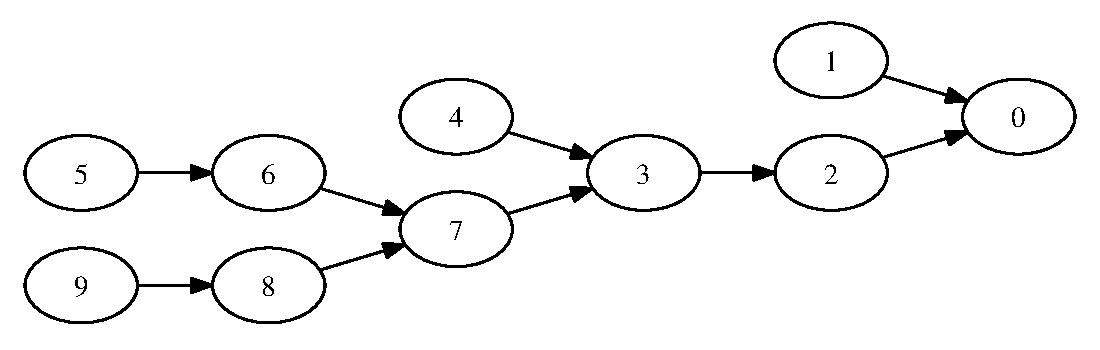
\includegraphics[scale=0.6]{figures/topo.eps}
\caption{汇聚树节点拓扑结构}\label{collection-tree}
\end{figure}

\subsubsection{CTP协议性能评价}
评价CTP协议的性能主要根据3个指标:开销,平均深度和包投递率。

{\kai 开销}是指平均每个单播包传输的总次数。由于包传输对节点来说所消耗的能量是相当可观的,因此开销的大小将直接影响到网络的生存时间,开销越大,网络的生存时间越短。它与路径的跳数,每个连接的重传数以及由于包丢失而造成的浪费有关。

{\kai 平均深度}指的是汇聚树的平均深度。如果所有的连接是完好的,没有重传和丢包,那么平均深度将是开销的下界。两者间的差异意味着选择连接的质量,这可能是由于重传或丢包所造成的,高效的路由算法可以使这个差异最小化。

{\kai 投递率}是指根节点收到的不重复消息的百分率,即根节点收到的数据包中除去重复的包所剩余的包数与所有节点发出的本地数据包数之比。这个指标的大小可以体现出丢包数,投递率越高说明丢包数越少。

在仿真结果中,可以通过监视节点转发引擎中的转发事件(包括了本地发送的包),计算出本地包的个数和转发次数。平均开销计算公式如下:
\begin{equation}
\text{\kai 平均开销} = \frac{\text{\kai 本地包发送次数} + \text{\kai 转发包发送次数}}{\text{\kai 本地包个数}}
\end{equation}
平均深度的计算就需要先获知汇聚树的拓扑结构,这可以通过监视父节点选择的变化获得。投递率的计算除了要监视转发事件之外,还需要监视根节点的包接收事件以得到投递成功的信息。根据上述方法对10个节点进行仿真,对比了使用标准LE和4BITLE的两种情况,得到表\ref{sim-result}所示结果:
\vspace{-5pt}
\begin{table}[ht]
\centering
\caption{\hei 仿真结果}\label{sim-result}
\vspace{5pt}
\wuhao
\begin{tabular}{l|rrr}
		& ~~~~~~~~标准LE& ~~~~~~~~4BITLE &增大消息缓存的4BITLE \\
\hline
转发包发送次数	&	3294 & 3002 & 3326 \\
本地包发送次数	&	1292 & 1272 & 1205 \\
本地包总个数	& 	121 & 120 & 124 \\
投递包个数(有重复)&	252 & 334 & 123 \\
投递包个数(去重复)&	109 & 115 & 117 \\
开销		&	37.90 & 35.62  & 36.54 \\
本均深度	&	2.0 & 2.9 & 3.5 \\
投递率		&	90.08\% & 95.83\% & 94.35 \\
\end{tabular}
\end{table}

从结果中可以看出,包发送的次数几乎是根节点实际接收到的包数的20$\sim$40倍,这是由于仿真使用的节点间连接质量(见表\ref{nodes-link-quality})设定的较差,导致节点间不断发生重传所造成的,这也是开销比平均深度大10$\sim$20倍左右的原因。但即便是在通信质量如此差的网络中,CTP协议还是可以成功地建立起多跳汇聚树,并保持了在90\%以上的较高的投递率,说明CTP协议是比较可靠的。

对比标准LE和4BITLE的数据可以发现,4BITLE即使在本均深度不如标准LE的情况下投递率还是明显高于标准LE的投递率,这是由于4BITLE使用了各层的信息得出的估计值比标准LE更精确,从而选择质量较差的连接的概率较小,丢包数也相应地减小。比较有重复的投递包个数和去重复的投递包个数可以发现,增大消息缓存后的4BILTE的包重复数(6个)远小于原来的4BITLE(219个),这是由于消息缓存的增大使节点存储已收到的包数增加,在缓存中停留的时间增长,从而发现重复包的概率增大。

\section{部署}
\subsection{自主开发节点简介}
实际部署的节点使用的是自主开发的npumote平台节点,它使用微处理器Atmega1281和无线模块RF230,配备了温湿度、光照等传感器,主要用于温室群的精准农业监控。

\subsection{为TinyOS 2.x添加平台支持}
由于TinyOS 2.x并没有直接支持我们的平台npumote,因而要对它做一些修改。主要的修改有如下几个方面:
\vspace{-10pt}
\begin{enumerate}
	\item{修改make系统:} 增加对avrisp2烧写器支持;增加npumote编译目标规则。
	\item{修改硬件参数和连接方式:} 修改串口的收发波特率;将AM层直接接到UniqueLayerC模块而不通过IEEE154网络层;增加EEPROM模块;修改RF230信道使程序在编译时可以通过增加RF230\_DEF\_CHANNEL标记设定信道值从EEPROM中读取;
\end{enumerate}
\vspace{-10pt}
将所有的改动以GNU diff格式记录到文件\texttt{npumote.patch}。在unix环境中,使用者只须将\texttt{npumote.patch}放在\texttt{tinyos-2.x}同一个目录下,进入\texttt{tinyos-2.x}目录, 执行命令:
\begin{lstlisting}[language=bash,numbers=none]
    patch -p1 <../npumote.patch
\end{lstlisting}
即可使TinyOS 2.x支持npumote平台。

\subsection{将程序烧写到节点中}
在使用CTP协议的应用程序源代码目录\texttt{apps/tests/TestNetwork}下运行以下命令将编译生成二进制文件并烧写到节点中:
\begin{lstlisting}[language=bash,numbers=none]
    make npumote install.<`节点号`> avrisp2,<`烧写器端口`>
\end{lstlisting}
如果编译通过但烧写失败,则需要检查烧写器端口是否书写正确并且确认当前用户是否具有该端口的读写权限。

\subsection{节点中程序的调试}
由于节点的资源有限,程序的调试相对比较困难。传统的做法是使用节点上的3个LED灯提供节点的状态信息。比如在节点启动完毕事件触发时,在程序中指定将红色的LED灯开启;在接收或发送消息时,使LED灯闪烁等方法得知节点的工作信息。这种方法是最实时有效的,但也是原始和效率低下的。TinyOS 2.x支持printf库的方法可通过串口向PC机发送调试信息,使调试方便了不少,但仍存在诸多限制,如在串口开启之前的调试信息无法发送,不能设置断点和查看更改寄存器信息,修改程序后要重新烧写节点等问题。另外,节点也可以使用JTAG硬件调试器调试,由于我们自主开发节点对这种方法的工具链支持还不完全,故不在此详述。总之,节点中程序的调试还有许多工作可以做,
可以作为以后研究工作的重点。

\subsection{节点部署}
节点号为0的节点在该应用程序中作为根节点使用,把它通过串口与上位机相连以便接收并处理汇聚上来的数据。其它节点的部署方法详见“无线传感器网络部署及其覆盖问题研究”\ucite{liuliping2006}。


% 结论
%%%%%%%%%%%%%%%%%%%%%%%%%%%%%%%%%%%%%%%%%%%%%%%%%%%%%%%%%%%%%%%%%%%%%%%%%
%
%   LaTeX File for Doctor (Master) Thesis of Tsinghua University
%   LaTeX + CJK     清华大学博士(硕士)论文模板
%   Based on Wang Tianshu's Template for XJTU
%	Version: 1.00
%   Last Update: 2003-09-12
%
%%%%%%%%%%%%%%%%%%%%%%%%%%%%%%%%%%%%%%%%%%%%%%%%%%%%%%%%%%%%%%%%%%%%%%%%%
%   Copyright 2002-2003  by  Lei Wang (BaconChina)       (bcpub@sina.com)
%%%%%%%%%%%%%%%%%%%%%%%%%%%%%%%%%%%%%%%%%%%%%%%%%%%%%%%%%%%%%%%%%%%%%%%%%

\renewcommand{\baselinestretch}{1.5}
\fontsize{12pt}{13pt}\selectfont

\chapter{总结与展望}\label{conclusion}
\markboth{总结与展望}{总结与展望}
%\addcontentsline{toc}{chapter}{\hei 总结与展望}
\section{全文总结}
汇聚协议是TinyOS中核心部分,理解汇聚协议对理解整个TinyOS架构有非常大的作用。本文使用自底向上的研究方法,循序渐进地分析了TinyOS 2.x中的CTP协议。主要做的工作如下:
\vspace{-10pt}
\begin{enumerate}
	\item 简述无线传感器网络体系结构,高度概括了节点的硬件特性、存在的限制和网络的组成形式。
	\item 简练地介绍了TinyOS操作系统的功能、特点和工作原理与nesC语言。
	\item 概述汇聚协议需要解决的问题,阐明TinyOS中CTP汇聚协议的总体架构,指出各部分之间的相互关联。
	\item 按照自底向上的顺序逐层分析CTP协议的基本原理。从最底层的链路估计器部分入手,讨论了两个节点间的链路质量估计方法,详细分析了基于LEEP帧探测的标准LE链路估计器,并简要描述了另一种更高效的链路估计方法4BITLE。
	\item 对中间层路由选择部分进行分析。探讨了路由引擎如何在节点资源受限的情况下高效地选择父节点的重要性,阐明了它选择下一跳所使用的路径ETX路由选择策略,同时也分析了路由协议工作的时序。
	\item 对上层的转发引擎进行分析。阐明了路由循环和包重复现象产生的原因,指出两者同时发生时对网络的不良影响,以及解决路由循环和抑制包重复的方法。另外解释了缓冲区分配的方法和缓冲区交换的设计意图。最后从本地包和转发包的发送这两方面指明转发引擎的工作流程。
	\item 对使用CTP协议的TinyOS应用程序的仿真作了详细的介绍,讲述了如何让节点在TOSSIM仿真中通信的方法,提出了一种可视化仿真的可行方案。接着分析仿真结果,给出仿真节点最终形成的拓扑结构。然后提出三个衡量汇聚协议性能的指标:开销、平均深度和投递率,并根据这几个指标对比使用标准LE估计器和4BITLE的性能差异,并简单分析了造成差异的原理。
	\item 描述将TinyOS移植到自主开发的节点平台npumote的方法,介绍了一些调试的心得,并对节点部署提出一些看法。
\end{enumerate}

\section{对未来工作的展望}
根据本文的分析,可以发现TinyOS中的CTP协议已经可以很好的工作,但也存在不少可以改进的地方,可以作为未来研究的重点,概括起来主要有如下几个方面:
\vspace{-10pt}
\begin{enumerate}
\item 可靠性问题。CTP协议对可靠性没有完全的保障。数据收集节点在向汇聚树中发送一个数据包后,不能得知该包是否被根节点接收和处理。因此,如果有实际应用要求绝对的可靠性,则CTP协议将不适用。如何以较小的代价为CTP增加应答机制以实现通信的可靠性,这是一个值得研究的问题。

\item 数据分片问题。CTP协议并不对发送的数据分片,如果有应用要求节点一次性收集发送的数据量较大(如视频采集),则CTP协议组成的网络吞吐率不高,很容易发生阻塞丢包现象。而对带宽有限的网络来说,超过带宽大小的数据包将无法发送。为CTP协议增加数据包分片机制是否能为网络性能带来提升,这也值得探讨。

\item 能耗问题。CTP协议没有考虑节点的能量剩余,这样可能使汇聚树中的一些通信量较大的节点率先从网络中消亡,从而减短了整个网络的生存期。如果将能量消耗问题考虑进去,在保证能通信的前提下平衡各个节点能耗,可能会使网络的生存时间上一个台阶。

\item 大规模节点通信。在节点数量大,分布过密的情况下,使用CTP协议的节点在启动初期网络中的广播通信量会异常的大,信道使用冲突现象很严重,从而影响节点正确地建立路由。可以寻找一种方法将这部分通信量按时间错开,以提高信道的利用率。另外,CTP协议由于资源限制使用的路由表较小,因此在邻居节点多的情况下可能连接质量最好的节点没有机会被选入路由表,从而使路由选择不能达到最优。如何使连接质量最好的节点必定能出现在路由表中,这也是具有研究的价值的。

\item 以数据为中心进行数据融合。CTP协议中的转发节点并不对转发数据作任何更改。但是在某些应用中,地理位置邻近的节点收集到的数据往往具有相关性,如果能在转发节点进行数据融合或数据筛选,将可以减少网络中的通信量,从而延长网络的生存时间。

\end{enumerate}


%参考文献
\wuhao

\bibliographystyle{unsrt}

\ifpdf \phantomsection \fi

\addcontentsline{toc}{chapter}{\hei 参考文献}

%\addtolength{\itemsep}{-0.8 em} % 缩小参考文献间的垂直间距, 在bibtex下无效
\bibliography{reference/reference}

% 致谢
%%%%%%%%%%%%%%%%%%%%%%%%%%%%%%%%%%%%%%%%%%%%%%%%%%%%%%%%%%%%%%%%%%%%%%%%%
%
%   LaTeX File for Doctor (Master) Thesis of Tsinghua University
%   LaTeX + CJK     清华大学博士(硕士)论文模板
%   Based on Wang Tianshu's Template for XJTU
%   Version: 1.00
%   Last Update: 2003-09-12
%
%%%%%%%%%%%%%%%%%%%%%%%%%%%%%%%%%%%%%%%%%%%%%%%%%%%%%%%%%%%%%%%%%%%%%%%%%
%   Copyright 2002-2003  by  Lei Wang (BaconChina)       (bcpub@sina.com)
%%%%%%%%%%%%%%%%%%%%%%%%%%%%%%%%%%%%%%%%%%%%%%%%%%%%%%%%%%%%%%%%%%%%%%%%%


%%%%%%%%%%%%%%%%%%%%%%%%%%%%%%%%%%%%%%%%%%%%%%%%%%%%%%%%%%%%%%%%%%%%%%%%%
%
%   LaTeX File for phd thesis of xi'an Jiao Tong University
%
%%%%%%%%%%%%%%%%%%%%%%%%%%%%%%%%%%%%%%%%%%%%%%%%%%%%%%%%%%%%%%%%%%%%%%%%%
%   Copyright 2002  by  Wang Tianshu    (tswang@asia.com)
%%%%%%%%%%%%%%%%%%%%%%%%%%%%%%%%%%%%%%%%%%%%%%%%%%%%%%%%%%%%%%%%%%%%%%%%%
\renewcommand{\baselinestretch}{1.5}
\fontsize{12pt}{13pt}\selectfont

\chapter*{致~~~~谢}
\markboth{致谢}{致谢}
\addcontentsline{toc}{chapter}{\hei 致谢}
首先要感谢我的导师李士宁教授。论文是在我的导师李老师的悉心指导下完成的。在论文的进展中,李老师提供了实验平台和学习资料,并且做了不少指点,对论文写作提出了很多宝贵意见。李老师严谨的治学态度以及丰富的实践经验将是我以后学习和工作的动力和楷模。在此谨向我的导师李士宁教授表示衷心的感谢。

同时要感谢传感器网络教研室李志刚老师和师兄师姐们,他们为我创造了良好的学习环境。他们提供的各种资料对我帮助很大,特别是林黛娣师姐在相同领域所作工作留下的资料使我受益匪浅。

另外要感谢UC Berkley的Philip Levis,USC的Omprakash Gnawali等人,是他们创造了TinyOS这个自由和优秀的WSN操作系统并提供了完整详细的文档;感谢为GNU/Linux贡献代码的黑客们,这个自由免费的平台为我完成毕设提供了不少便利;感谢清华大学王磊博士,他创作的\LaTeX 模板使我的论文的排版得以顺利完成。

最后感谢我的家人对我一如既往的关心和支持,感谢即将出世的侄儿给我带来精神上莫大的鼓舞。

\chapter*{毕业设计小结}
\markboth{毕业设计小结}{毕业设计小结}
\addcontentsline{toc}{chapter}{\hei 毕业设计小结}

这次毕业设计是对我四年本科学习的一个总结,涉及了操作系统、计算机网络、体系结构、组成原理等课程的知识,并且要求自己动手实践,这对我来说是一次全面的考验。一开始对于TinyOS和nesC语言完全是陌生的,对组件化设计的概念理解也不够深入。接着是各种安装和配置问题,只能通过官方的教程和TinyOS的邮件列表查询,信息的来源比较少。由于nesC并不是一种广泛使用的语言,因此各种相关的工具比较少,比如没有优秀的可视化工具可用,从而导致阅读TinyOS代码相对比较困难:为了找一个命令的实现,需要顺着配置文件层层挖掘,有时甚至要深入十几层才能找到具体实现的代码,后来通过自定义配置编辑器以及查找辅助工具才略微提高了一些效率,这一过程颇为坎坷。

本次毕业设计中印象比较深刻的是节点上程序的调试,节点没有足够的资源用于支持断点,甚至获知节点的当前运行状态也是相当困难的,通过串口的调试信息并不一定是实时的,因而只能通过节点上的3个LED灯得知准确状态信息,这是以后可以改进的地方。

经历了本次毕设,我对无线传感器网络有了一定的了解,积累了一些实际经验,对以后研究生阶段的学习目标也更加明确了。





%  附录

%\begin{appendix}
%    \renewcommand{\chaptername}{附录\Alph{chapter}}
%   \chapter*{附~~录}
\markboth{附录}{附录}
\addcontentsline{toc}{chapter}{\hei 附录}
\noindent\bfseries\texttt{test.py}源代码:
\setmonofont{Monaco}
\lstset{basicstyle=\ttfamily\scriptsize,keywordstyle=\color{blue},commentstyle=\color{green},stringstyle=\color{red},tabsize=4,frameround=fttt,escapeinside=``,lineskip=0.6pt}
\begin{lstlisting}[language=Python]
#!/usr/bin/env python
from TOSSIM import *
from random import *
import sys

if len(sys.argv) < 3:
	print "usage: need 2 parameter, nodes number and simulate time"
	sys.exit(0)

nodes = int(sys.argv[1])
sim_time = int(sys.argv[2])
t = Tossim([])
r = t.radio()

f = open("topo.txt", "r")
lines = f.readlines()
for line in lines:
  s = line.split()
  if (len(s) > 0):
    if s[0] == "gain":
      r.add(int(s[1]), int(s[2]), float(s[3]))

noise = open("meyer-short.txt", "r")
lines = noise.readlines()
for line in lines:
  str = line.strip()
  if (str != ""):
    val = int(str)
    for i in range(0, nodes):
      m = t.getNode(i);
      m.addNoiseTraceReading(val)

for i in range(0, nodes):
  m = t.getNode(i);
  m.createNoiseModel();
  time = randint(t.ticksPerSecond(), 10 * t.ticksPerSecond())
  m.bootAtTime(time)
  print "Booting ", i, " at time ", time

print "Starting simulation."

t.addChannel("Forwarder", sys.stdout)
t.addChannel("TestNetworkC", sys.stdout)
t.addChannel("TreeRouting", sys.stdout)
t.addChannel("LI", sys.stdout)

while (t.time() < sim_time):
  t.runNextEvent()

print "Completed simulation."
\end{lstlisting}

\noindent\bfseries\texttt{ctpsim-3d.py}源代码:
\begin{lstlisting}[language=Python,tabsize=2]
#!/usr/bin/env python
import xmlrpclib,time
import re

nodes = 10
server = xmlrpclib.Server('http://localhost:20738/RPC2')
G = server.ubigraph

G.clear()

node = [0 for col in range(nodes)]

for i in range(0,nodes):
	node[i] = G.new_vertex()
	G.set_vertex_attribute(node[i], 'label', str(i))
	G.set_vertex_attribute(node[i], 'shape','sphere')
	G.set_vertex_attribute(node[i], 'size','0.5')
	G.set_vertex_attribute(node[i], 'color','#1E90FF')

edge = [[0 for col in range(nodes)] for row in range(nodes)]

for i in range(0,nodes):
	for j in range(i+1, nodes):
		edge[i][j] = G.new_edge(node[i], node[j])
		edge[j][i] = edge[i][j]

topo = open('topo.txt', 'r')
lines = topo.readlines()
for line in lines:
	s = line.split()
	if s[0] == 'gain':
		if int(s[1]) < nodes and int(s[2]) < 
				nodes and int(s[1]) < int(s[2]):
			G.set_edge_attribute(edge[int(s[1])][int(s[2])],
					     'strength',
					     str(1 + float(s[3]) / 120.0))
			#G.set_edge_attribute(edge[int(s[1])][int(s[2])],
					      'label', s[3]) # add gain value

G.set_vertex_attribute(node[0], 'color', '#FFFF00') # root node

def node_spark(node_id):
	node_id = int(node_id)
	G.set_vertex_attribute(node[node_id], 'color', '#FF0000')
	G.set_vertex_attribute(node[node_id], 'color', '#FFFFFF')
	G.set_vertex_attribute(node[node_id], 'color', '#FF0000')
	G.set_vertex_attribute(node[node_id], 'color', '#FFFFFF')
	if node_id != 0:
		G.set_vertex_attribute(node[node_id], 'color', '#1E90FF')
	else:
		G.set_vertex_attribute(node[node_id], 'color', '#FFFF00')


def node_display_debug_str(node_id, debug_str):
	G.set_vertex_attribute(node[int(node_id)], 'label', node_id+": "+debug_str)
	#time.sleep(0.0)
	#G.set_vertex_attribute(node[node_id], 'label', str(node_id))

def process_boot_at_time(node_id, time):
	G.set_vertex_attribute(node[int(node_id)], 'label','boot at:'+time)


def process_parent_change(node_id, origin_parent, new_parent):
	node_id = int(node_id)
	origin_parent = int(origin_parent)
	new_parent = int(new_parent)
	if origin_parent != 65535:
		G.set_edge_attribute(edge[node_id][origin_parent], 'color', '#C0C0C0')
		G.set_edge_attribute(edge[node_id][origin_parent], 'width','1')
	G.set_edge_attribute(edge[node_id][new_parent], 'color', '#FF00FF')
	G.set_edge_attribute(edge[node_id][new_parent], 'width','7')
	time.sleep(0.5)

def animateArrow(e, reverse):
  pos = 0.0
  if reverse:
    pos = 1.0
  G.set_edge_attribute(e, "arrow_position", str(pos))
  G.set_edge_attribute(e, "arrow_reverse", str(reverse))
  G.set_edge_attribute(e, "arrow", "true")
  for i in range(0,20):
    a = i / 19.0
    if reverse:
      a = 1.0 - a
    G.set_edge_attribute(e, "arrow_position", str(a))
    time.sleep(0.05)
  G.set_edge_attribute(e, "arrow", "false")

def animate_broadcast(node_id):
	node_id = int(node_id)
	for j in range(2):
		for i in range(21):
			G.set_vertex_attribute(node[node_id], 
				'size', str(0.5 + i / 20.0))
		for i in range(21):
			G.set_vertex_attribute(node[node_id],
				'size', str(0.5 + (20 - i)/20.0))

def process_send_beacon(node_id):
	node_id = int(node_id)
	animate_broadcast(node_id)
	

def process_forwoard_subsend(node_id, dest):
	print node_id, dest
	node_id = int(node_id)
	dest = int(dest)
	if node_id == dest:
		return
	G.set_edge_attribute(edge[node_id][dest], 'arrow','true')
	if node_id > dest:
		G.set_edge_attribute(edge[node_id][dest], "arrow_reverse", 'true')
	speed = 10 # the smaller, the faster
	for pos in range(speed+1):
			if node_id < dest:
				G.set_edge_attribute(edge[node_id][dest], 
					"arrow_position", str(pos / float(speed)))
			else:
				G.set_edge_attribute(edge[node_id][dest], 
					"arrow_position", str(1- pos / float(speed)))
			time.sleep(0.05)
	G.set_edge_attribute(edge[node_id][dest], "arrow_reverse", 'false')
	G.set_edge_attribute(edge[node_id][dest], 'arrow','false')

def dispatch_each_line(line):
	re_boot_at_time = r'Booting  (/d+)  at time  (/d+)'
	re_debug = r'^DEBUG \((\d+)\): (.*)'

	re_parent_change = r'Changed parent. from (\d+) to (\d+)'
	# 1.parent,  2.etx
	re_send_beacon = r'CtpRoutingEngineP\$0\$sendBeaconTask\$runTask parent: (\d+) etx: (\d+)' 
	# 1.dest, 2. error
	re_forward_subsend = r'CtpForwardingEngineP\$0\$SubSend\$sendDone to (\d+) and (\d+)' 

	match = re.match(re_boot_at_time, line)
	if match:
		process_boot_at_time(match.group(1), match.group(2))
	else:	# match debug messages
		match = re.match(re_debug, line)
		if match:
			node_id = match.group(1)
			node_spark(node_id)
			debug_str = match.group(2)
			node_display_debug_str(node_id, debug_str)
			
			if re.match(re_parent_change, debug_str):
				match = re.match(re_parent_change, debug_str)
				process_parent_change(node_id, match.group(1), match.group(2))
			elif re.match(re_send_beacon, debug_str):
				process_send_beacon(node_id)
			elif re.match(re_forward_subsend, debug_str):	# Forwarder send a packet
				match = re.match(re_forward_subsend, debug_str)
				process_forwoard_subsend(node_id, match.group(1))
line = raw_input()
while line:
	dispatch_each_line(line)
	line = raw_input()
\end{lstlisting}

%\end{appendix}

% 发表的文章列表

%\include{appendix/publications}

\clearpage
\end{document}

%%%%%%%%%%%%%%%%%% End of the file  %%%%%%%%%%%%%%%%%%%%%%%%
